\documentclass[conference]{IEEEtran}

% Make latex understand and use the typographic
% rules of the language used in the document.
\usepackage[english]{babel}
\usepackage[utf8]{inputenc}
% Choose the font encoding
\usepackage[T1]{fontenc}

% Use colour in tables
\usepackage[table]{xcolor}
\usepackage{array}
\usepackage{multirow}

% load a colour package
\usepackage{xcolor}
\definecolor{aaublue}{RGB}{33,26,82}% dark blue

% The standard graphics inclusion package
\definecolor{white}{RGB}{255,255,255} % define color white
\usepackage{graphicx}

% Set up how figure and table captions are displayed
\usepackage{caption}
\captionsetup{
  font=footnotesize,% set font size to footnotesize
  labelfont=bf % bold label (e.g., Figure 3.2) font
}

% Enable row combination in tables
\usepackage{multirow}

% Make space between table lines and text
\renewcommand{\arraystretch}{1.5}

% Make the standard latex tables look so much better
\usepackage{array,booktabs}



%%%%%%%%%%%%%%%%%%%%%%%%%%%%%%%%%%%%%%%%%%%%%%%%
% Mathematics
%%%%%%%%%%%%%%%%%%%%%%%%%%%%%%%%%%%%%%%%%%%%%%%%
% Defines new environments such as equation,
% align and split 
\usepackage{amsmath}
\usepackage{relsize}
% Adds new math symbols
\usepackage{amssymb}
% Use theorems in your document
% The ntheorem package is also used for the example environment
% When using thmmarks, amsmath must be an option as well. Otherwise \eqref doesn't work anymore.
\usepackage[framed,amsmath,thmmarks]{ntheorem}
\usepackage{cancel}

%%%%%%%%%%%%%%%%%%%%%%%%%%%%%%%%%%%%%%%%%%%%%%%%
% Page Layout
%%%%%%%%%%%%%%%%%%%%%%%%%%%%%%%%%%%%%%%%%%%%%%%%


%%%%%%%%%%%%%%%%%%%%%%%%%%%%%%%%%%%%%%%%%%%%%%%%
% Bibliography
%%%%%%%%%%%%%%%%%%%%%%%%%%%%%%%%%%%%%%%%%%%%%%%%
%%setting references (using numbers) and supporting i.a. Chicargo-style:
\usepackage{etex}
\usepackage{etoolbox}
\usepackage{keyval}
\usepackage{ifthen}
\usepackage{url}
\usepackage{csquotes}
\usepackage[backend=biber, url=true, doi=true, citestyle=ieee, bibstyle=ieee, sorting=none]{biblatex}
\addbibresource{setup/bibliography.bib}

%%%%%%%%%%%%%%%%%%%%%%%%%%%%%%%%%%%%%%%%%%%%%%%%
% Misc
%%%%%%%%%%%%%%%%%%%%%%%%%%%%%%%%%%%%%%%%%%%%%%%%

%%% Enables the use FiXme refferences. Syntax: \fxnote{...} %%%
\usepackage[footnote, draft, english, silent, nomargin]{fixme}
%With "final" instead of "draft" an error will ocure for every FiXme under compilation.

%%% allows use of lorem ipsum (generate i.e. pagagraph 1 to 5 with \lipsum[1-5]) %%%
\usepackage{lipsum}

%%% Enables figures with text wrapped tightly around it %%%
\usepackage{wrapfig}

\usepackage{float}
\usepackage{caption}
\usepackage{subcaption}
\usepackage{siunitx}
\sisetup{decimalsymbol=comma}
\sisetup{detect-weight}

\usepackage{enumitem}
%\usepackage[citestyle=authoryear,natbib=true]{biblatex}

% Figures - TIKZ
\usepackage{tikz}
\usetikzlibrary{shapes,arrows}
\usepackage[americanresistors,americaninductors,americancurrents, americanvoltages]{circuitikz}

% Wall of text logo
\newcommand{\walloftextalert}[0]{\includegraphics[width=\textwidth]{walloftext.png}}

\usepackage{pdfpages}
\usepackage{lastpage}
\usepackage{epstopdf}

\setlength{\headheight}{21pt}

\hfuzz=\maxdimen
\tolerance = 10000
\hbadness  = 10000

\usepackage{siunitx}
\graphicspath{{./figures/}}% package inclusion and set up of the document

%%%%%%%%%%%%%%%%%%%%%%%%%%%%%%%%%%%%%%%%%%%%%%%%%%%%%
%             UNITS, EQUATIONS AND TEXT             %
%%%%%%%%%%%%%%%%%%%%%%%%%%%%%%%%%%%%%%%%%%%%%%%%%%%%%
%Units:
\newcommand{\unit}[1]{&& \left[\si{#1}\right]} %\newcommand{\unit}[1]{[\si{#1}]}             <<| Use these if you want uations to be
\newcommand{\unitWh}[1]{[\si{#1}]}             %\newcommand{\eq}[2]{&&\si{#1} &= \si{#2}&&}  <<| centered.. .. will appear scrambled
\newcommand{\numUnit}[1]{\ \si{#1}&}           %                                               | from one equation to the next though..
%Equation:                                     %                                               | and does not work with long equations.. :/
\newcommand{\eq}[2]{\si{#1} &= \si{#2}}
\newcommand{\arw}{&& &\Updownarrow&&}
\newcommand{\eqOne}[2]{\si{#1} &= \si{#2} &\nonumber\\}
\newcommand{\eqTwo}[1]{&\ \ \ \ \si{#1}& \nonumber\\}
\newcommand{\eqThree}[1]{&\ \ \ \ \si{#1}&}
%Text:
\newcommand{\tx}[1]{\text{#1}}
%Vectors
\renewcommand{\vec}[1]{\boldsymbol{\mathbf{#1}}}
%Vertical line in equations ie. |_x=y (whereTwo stacks two equalities at the line)
\newcommand{\lineWhere}[1]{ \left.\rule{0cm}{.5cm}\right\vert\rule{0cm}{.4cm}_{\substack{\rule{0cm}{.15cm}\\ \si{#1} }} }
\newcommand{\lineWhereTwo}[2]{ \left.\rule{0cm}{.67cm}\right\vert\rule{0cm}{.5cm}_{\substack{\si{#1} \rule{0cm}{.19cm}\\\vspace{-.1cm}\\ \si{#2}}} }

%%%%%%%%%%%%%%%%%%%%%%%%%%%%%%%%%%%%%%%%%%%%%%%%%%%%%
%                 TIKZ SETTINGS                     %
%%%%%%%%%%%%%%%%%%%%%%%%%%%%%%%%%%%%%%%%%%%%%%%%%%%%%
%\usetikzlibrary{arrows.meta}
\tikzset{
  block/.style    = {draw, thick, rectangle,
                     minimum height = 2.1em,
                     minimum width = 1.7em},
  sum/.style      = {draw, circle, inner sep=1.5pt},
}

%%%%%%%%%%%%%%%%%%%%%%%%%%%%%%%%%%%%%%%%%%%%%%%%%%%%%
%               WHERE, AFTER MATH                   %
%%%%%%%%%%%%%%%%%%%%%%%%%%%%%%%%%%%%%%%%%%%%%%%%%%%%%
\usepackage{xifthen}

\newenvironment{where}{\par\vspace{-4mm}\noindent\ignorespaces Where:\\}{\\}
\newcommand{\va}[3]
{
  \begin{tabular}{p{10pt} p{145pt} l}
    { $#1$ } & { #2 } & \ifthenelse{\isempty{ #3 }}  {}  {[{\si{#3}}]} \\
  \end{tabular}\\
}% my new macros

%\toggleNotes{on}

\begin{document}
	%%% Prereport %%%
	\setlength\cftaftertoctitleskip{2pt}
	\setlength\cftafterloftitleskip{6pt}
	\setlength\cftafterlottitleskip{6pt}
	\selectlanguage{english}
	\title{Quadcopter}
	
	%%% Frontmatter Settings %%%
	\pagestyle{empty} %disable headers and footers
	\pagenumbering{roman} %use roman page numbering in the frontmatter I II...
	\fancyfoot[RE,LO]{16gr733} %page number on all pages
	\fancyfoot[LE,RO]{\thepage}
	\fancyhead[LE,LO,RE,RO]{}
	
	%%% Introductory Formalities %%%
	\pdfbookmark[0]{Front Page}{label:forside}%
\begin{titlepage}
  \addtolength{\hoffset}{0.5\evensidemargin-0.5\oddsidemargin} %set equal margins on the frontpage - remove this line if you want default margins
  \noindent%
  \begin{tabular}{@{}p{\textwidth}@{}}
    \toprule[2pt]
    \midrule
    \vspace{0.2cm}
    \begin{center}
    \Huge{\textbf{
      Attitude and Position Control of a Quadcopter in a Networked Distributed System}}
    \end{center}
	\vspace{0.19cm} \\
    \midrule
    \toprule[2pt]
  \end{tabular}
   \vspace{0.23 cm}
  \begin{figure}[!ht]
\centering
\includegraphics[width=0.75\textwidth]{figures/FrontPageCropped}
\label{fig:forside}
\end{figure}
  \vspace{-0.6 cm}
  \begin{center}
    {\large
      1. Semester Project Worksheets %Insert document type (e.g., Project Report)
    }\\
    \vspace{0.1 cm}
    {\Large
      Group 16gr733%Insert your group name or real names here
    }
  \end{center}
  \vspace{-0.45 cm}
  \begin{center}
  Aalborg University\\
  Automation and Control\\
  Fredrik Bajers Vej 7\\
  DK-9220 Aalborg
  \end{center}
\end{titlepage}

\clearpage
	\pagestyle{fancy}
	\input{formalities/kolofon}
	%\begin{document} 
%\thispagestyle{empty}
%\begin{titlepage}
\begin{nopagebreak}
{\samepage 

\begin{tabular}{r}
\parbox{\textwidth}{  \raisebox{-15mm}{\includegraphics[height=3cm]{figures/aaulogo-en.png}}
\hfill \hspace{2cm} \parbox{8cm}{\begin{tabular}{l} %4.90
{\small \textbf{\textcolor{aaublue}{\colorbox{white}{1\textsuperscript{st} Semester Project}}}}\\
{\small \textbf{\textcolor{aaublue}{Master's Program}}}\\ 
{\small \textbf{\textcolor{aaublue}{Control and Automation}}}\\ 
{\small \textcolor{aaublue}{Department of Electronic Systems}}\\
{\small \textcolor{aaublue}{Fredrik Bajers Vej 7C, 9220 Aalborg}} \\
 \\
%{\small \textcolor{aaublue}{\emph{http://www.sict.aau.dk/electronics-and-it}}}
\end{tabular}}}
\end{tabular}

\begin{tabular}{cc}
\parbox{7cm}{

\textbf{Title:}

Attitude and Position Control\\ of a Quadcopter in a \\Networked Distributed System \\

\textbf{Theme:} \\
\small{Networked Control Systems
\\
}


\parbox{8cm}{


\textbf{Project Period:}\\
Fall 2016\\
%01/09/2016 - 20/12/2016\\
   
\textbf{Project Group:}\\
733\\ %\fxnote{Input group number}
  
\textbf{Participants:}\\
Alejandro Alonso García\\
Amalie Vistoft Petersen\\
Andrea Victoria Tram Løvemærke\\
Niels Skov Vestergaard\\
Noelia Villarmarzo Arruñada\\

\textbf{Supervisor:}\\
}\\Anders la Cour-Harbo


\textbf{Pages:} 125\fxnote{PAGES}\\
\textbf{Appendices:}\fxnote{PAGES} 6 (37 pages)\\
\textbf{Attachments:} 1 \\
\textbf{Concluded:} 20/12/2016\\

\vfill } &
\parbox{7cm}{
  \vspace{.15cm}
  \hfill
  \begin{tabular}{l}
  {\textbf{Synopsis}}\bigskip \\
  \fbox{
    \parbox{6.5cm}{\bigskip
     {\vfill{\small \input{formalities/synopsis.tex}
     \bigskip}}
     }}
   \end{tabular}}
\end{tabular} %\vspace{1cm}
}


\textit{\phantom{A}Publication of this report's contents (including citation) without permission\\ \phantom{A}from the authors is prohibited}\\

\end{nopagebreak}
%\end{titlepage}
%\end{document}
	%%% Preface %%%
	%\cleardoublepage
	\newgeometry{left=25mm,	right=25mm, top=18mm}

\chapter*{Preface}
%\textbf{\huge{Preface}}
This P1 project of the Control and Automation master program at Aalborg University has been carried out in the fall 2016 by the student group 16gr733. 
The focus of this project is to make a quadcopter stable and control its position in a distributed networked system. 
It is expected of the reader to have knowledge within mathematics and physics as well as electronics and linear control theory.
For referencing sources the standard ISO 690 is used, noting [n], where n represents a number in the bibliography. The bibliography is placed at the end of the worksheets, before appendices. Additional attachments are uploade along with the worksheets, these are code-files, MATLAB simulation scrips, online sources, and the paper and poster for this project.   

Anders la Cour-Harbo, associate professor at Aalborg University, has been the supervising the project. 

Aalborg University deserves a thank you for providing the quadcopter. A thank should also be given to Jesper D. Pedersen, industrial technician at Aalborg University, for building test setups for the quadcopter. 

Lastly Henrik Shøiler, associated professor at Aalborg University, must be acknowledge for his assistance in the labratory and kind sharing of implementational experiences.

\textbf{Text by:}\\
\vspace{-5pt}
\begin{table}[H]
	\centering
		\begin{tabular}{c c c}
			\underline{\phantom{JAERJAERJAERJAERGO}} & \phantom{cookies} & \underline{\phantom{JAERJAERJAERJAERGO}} \\
			Alejandro Alonso García			& \phantom{cookies} & Amalie Vistoft Petersen		\\
			&&\\
			\underline{\phantom{JAERJAERJAERJAERGO}} & \phantom{cookies} & \underline{\phantom{JAERJAERJAERJAERGO}} \\
			Andrea Victoria Tram Løvemærke			& \phantom{cookies} & Niels Skov Vestergaard		\\
			&&\\
	    \multicolumn{3}{c}{\underline{\phantom{JAERJAERJAERJAERGO}}}\\
	    \multicolumn{3}{c}{Noelia Villarmarzo Arruñada}\\				
		\end{tabular}
\end{table}

\pagebreak
\restoregeometry
	
	\restoregeometry

%\restoregeometry

\pdfbookmark[0]{TableofContent}{label:Indhold}
\tableofcontents

%\printglossary[title=List of Terms,toctitle=Terms and abbreviations,type=\acronymtype]

%\glsaddall
%\printglossary
%\printglossary[type=\acronymtype]




\cleardoublepage
	
	%%% Mainmatter Settings %%%
	\pagenumbering{arabic} %use arabic page numbering in the mainmatter
	\fancyfoot[RO,LE]{\thepage \text{ of} \pageref{LastPage}}
	\fancyfoot[RE,LO]{16gr733}
	\fancyhead[RE,LO]{}
	\fancyhead[RE,LO]{\color{aaublue}\small\nouppercase\leftmark} %even page - chapter title
	\pagestyle{fancy}
	
	%%% Part 1 %%%
	\part{Preliminary Analysis}
	
	%---------- Chapter 1 ---------------------------------------- 
	\chapter{Introduction}
Drones has a wide variety of potential uses, such as search and rescue, inspection, security, surveillance, research, aerial photography, unmanned cargo systems, military applications, the list goes on. Drones are already widely used, and while some of the aforementioned applications raises ethical issues for debate, there is no doubt that drones also hold a place in the future.

Multicopters constitutes a class of drones with fixed-pitch propellers. This means that the actuation is achieved from a difference in speed between the propellers. Among the all the different varieties of multicopters, see some examples on \autoref{fig:multicopters}, the quadcopter is the most popular, largely due to a compromise between stabilization capabilities and cost of hardware. \cite{TypesOfMulticopter}

\begin{figure}[H]
  \centering
  \includegraphics[width=.6\linewidth]{figures/multicopters}
  \caption{A small selection of drones which belongs to the large class of multicopters. \cite{multiCopterPhoto}}
  \label{fig:multicopters}
\end{figure}

The aim of the project is to investigate the capabilities of a specific design strategy when controlling the attitude of a quadcopter as part of a distributed system.

The quadcopter obtains its attitude over a network from a motion tracking system. This introduces delay and packet loss as a limiting factor to the control system situated on the quadcopter. The controlling code is implemented in C on a microcontroller using a real time operating system (RTOS), called FreeRTOS.

The system's coupled behavior and instability raises a challenging control task. This task is solved by implementing a controller design, which is based upon a model that is derived by first principle modeling. This is later linearized since it is desired to use linear controllers.\\
The system is divided into an attitude controller and translational controllers. The attitude controller is in focus in this project. The translational controllers are cascaded around the attitude controller.

The attitude control strategy is based in state space design, and makes use of state feedback, a linear quadratic regulator (LQR) and an integral controller.\\
The translational controllers are designed as classical proportional and integral controllers around the inner state space design.
	
	%---------- Chapter 2 ---------------------------------------- 
	\chapter{System Description}
In this project a quadcopter is provided with motors, motor controllers, propellers and a battery. The system in its initial state is seen on \autoref{fig:systemBase}. Apart from the quadcopter and the attached hardware, a tracking system called Vicon is also provided. This is used to track the quadcopter and provide it with sensor inputs.

Additional to the provided hardware, an ATmega 2560 and XBEE modules are used as a processor and wireless communication modules, respectively.

\begin{figure}[H]
  \centering
  \includegraphics[width=.6\linewidth]{figures/quadcopterBaseLabels}
  \caption{The quadcopter with attached hardware as given.}
  \label{fig:systemBase}
\end{figure}

In this chapter the hardware is presented after which the overall structure of the prototype is described.
	\section{Hardware}\label{sec:hardware}
%The quadcopter has been provided by Aalborg university and professor Henrik Shjøiler\fixme{add danish letters}. This chapter has the purpose of describing the hardware. 
%The hardware is tested and the results of these test will be presented. 
The hardware used to develop this project consists of the quadcopter and the Vicon system that is used as a sensor. In this section, the most relevant hardware is explained in more detail. \cite{YDing}

\subsection{Motor and Propeller}
The quadcopter is equipped with four brushless outrunner motors named Turnigy Multistar. 

Brushless motors are electric powered with a DC power that require a electronic commutator, which generates a sinusoidal or trapezoidal waveform, to run the motor. They have a higher power density and higher reliability than conventional DC motors.

Within this kind, outrunner motors have their magnets in the outer shell, the rotor. The rotor spins around the fixed coils that form the stator. Due to the more space in the rotor for magnets, they normally have more poles that inrunner motors, and thus, are able to produce more torque for the same size.  

The motor used has a $k_v$ of 935 $rpm/V$, 14 poles and maximum current of 15 $A$ \cite{HkingPropeller}.

The motor used is shown in \autoref{fig:Motor}.
\begin{figure}[H]
	\centering
	\includegraphics[scale=0.5]{figures/motor.png}
	\caption{One of the four motors mounted on the quadcopter.}
	\label{fig:Motor}
\end{figure} 

The propellers are sold with the motors and are 10 inches long (25.4 cm) and has a pitch of 4.5 (11,43 cm) inches. The pitch is the distance traveled by a propeller after one complete rotation. For this to be true the propeller must turn inside a solid surface, the traveled distance is less if it rotates inside a liquid or gas \cite{EReyes}. A higher pitch creates more turbulence and make the quadcopter less steady when flying \cite{oscarliang}.

The length of the propeller is proportional to the efficiency of the quadcopter. Hence, a longer propeller has an increase in maximum speed. The acceleration of a small propeller is greater than that of a larger propeller. Thus it is easier to change the inertia of moment if utilizing a small propeller compared to a larger one. \cite{oscarliang}

In this case a propeller which is 10 inches long and has a pitch of 4.5 is suitable for the utilized quadcopter, as it has been utilized in multiple cases before. 

A picture of the utilized propellers can be seen in \autoref{fig:Propeller}.

\begin{figure}[H]
	\centering
	\includegraphics[scale=0.4]{figures/propeller.png}
	\caption{Two of the four propellers mounted on the quadcopter's motors.}
	\label{fig:Propeller}
\end{figure}

%The relationship between PWM signal to the motor controllers and the velocity of the propeller can be seen in Figure ZZ. \fxnote{pull diagram from measurement report}

%It has been observed during tests, that the motor runs faster as it's temperature increases. This is not expected due to the increased resistance, that occurs when the coils within the motor are heated. Therefore the relationship between PWM signal and velocity is not representative for all cases. It is however deemed reasonable to neglect this variance and presume a relationship as it is derived in the measurement report, see Appendix YY.
 
\subsection{Motor Controller}
The quadcopter comes with four electronic speed controllers, ESCs, one for each motor. The ESCs produce an 8 kHz PWM, are rated for a 2-4 cell Li-Po battery and can handle a constant current of up to 30 A. The ESCs also has a 5.5 V, 4 A output for powering e.g. a controller board.\cite{HKing}

\begin{figure}[H]
	\centering
	\includegraphics[scale=0.4]{figures/ESC}
	\caption{One of the four Electronic Speed Controllers mounted on the quadcopter.\cite{HKing}}
	\label{fig:esc}
\end{figure}
\subsection{Processor}
The implementation of the controllers is done in a microprocessor from Atmel, the ATmega2560, mounted in the ArduinoMEGA development board, as seen in figure \autoref{fig:ATmega}.

This processor has up to 16 PWM output channels, two 8-bit timers and four 16-bit timers, four USART modules, 8 kilobytes of internal memory and a processing speed of 16 MIPS. With this capabilities, a quadcopter control could be implemented.

The use of the development board makes the use of the wireless modules easier as an arduino shield can be directly plugged in. Furthermore, it allows a faster set up of the microcontroller as all required hardware (oscillatior, power supply, etc.) is already present in the board. 
\begin{figure}[H]
	\centering
	\includegraphics[scale=0.17]{figures/ARDUINO_MEGA}
	\caption{AtMega2560 mounted in the ArduinoMEGA development board.}
	\label{fig:ATmega}
\end{figure}
\subsection{Wireless Modules}
The wireless modules used to communicate with the quadcopter are called XBEE, see \autoref{fig:XBEE}. They communicate at a 2.4 GHz frequency and they take care of all communication layers but the transport layer protocol. In order to use this modules, the packet has to be sent through the serial port when using the computer or through the USART module when using the microcontroller. 
\begin{figure}[H]
	\centering
	\includegraphics[scale=0.4]{figures/XBEE}
	\caption{XBEE wireless modules.}
	\label{fig:XBEE}
\end{figure}

\subsection{Battery}
The battery available for the prototype, is a Zippy Flightmax battery. It weighs 141 gram, has a capacity of 1500 mAh, a voltage of 11.1 volts and a discharge current of 20 amperes.

%removed by Niels: It shall be noted, that the battery level...
The battery level drops over time, with a significance that can not be neglected as it may have great impact on the output of the motor and therefore on the lift of the propeller. It is possible to measure the battery level while operating the quadrotor. By taking into account the battery level in the test of the PWM signal to velocity, it is possible to obtain a quadcopter having constant lift force, if this is requested\fxnote{Niels and Alejandro suggest: With this information and knowledge of the relationship between voltage and RPM it is possible to account for the battery level, and thereby rectify the problem. [ref to test - maybe - should the test be discussed this early?]}.

\subsection{Vicon System}
The Vicon system is a powerful tool that provides real-time position and orientation data captured with 9 infrared cameras.This information can be used to track objects inside the room the system is built in.
%An example is found in Aalborg University as seen in \figref{ViconRoom}. 

%\begin{figure}[H]
%	\centering
%	\includegraphics[scale=0.5]{figures/ViconRoom}
%	\caption{Aalborg University's Vicon room.}
%	\label{ViconRoom}
%\end{figure}

To use this system, markers are attached to the object that is to be tracked. The Vicon system streams the position of the markers and the position and orientation of the object at 100 Hz for a computer to read them. The data can be received by using an SDK plugin for MATLAB. In this way, data can be operated in the MATLAB environment, making it easier to obtain variable derivatives like velocities or accelerations.

The user interface of the Vicon system is shown in \autoref{fig:ViconTracker}. 
\begin{figure}[H]
	\centering
	\includegraphics[scale=0.27]{figures/ViconTracker}
	\caption{User interface of the Vicon System, the Vicon Tracker. An object has been created from the markers placed on the drone.}
	\label{fig:ViconTracker}
\end{figure}
It is called Vicon Tracker and it allows the creation of objects by grouping markers present in the room. It also allows to change the center of gravity of the created objects and rotate the inertial and body reference frames to any desired orientation.		
	\section{Prototype Description}
In the following section an overall description of the prototype is given. This is done to help the reader understand the utilized setup in the project.
The prototype is divided into 3 separate subsystems. The quadcopter, the ground station and the vicon system. These subsystems can be seen in \figref{prototypediagram}. 

\begin{figure}[H] 
	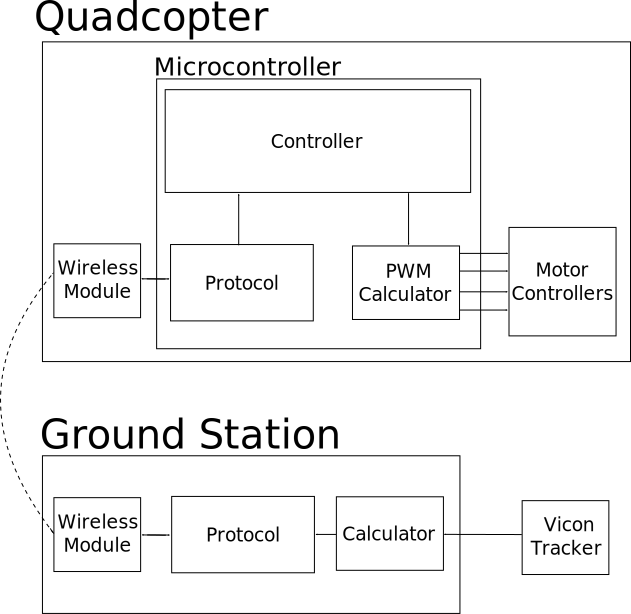
\includegraphics[scale=.5]{figures/prototypediagram}
	\centering
	\captionsetup{justification=centering}
	\captionof{figure}{Schematic diagram of the prototype, which includes the quadcopter, the ground station and the vicon system.}
	\label{prototypediagram}
\end{figure}

\todo{explain somewhere what vicon is and that it can be found in aalborg university, maybe we should have a little section?.}

For this project the Vicon system is utilized to capture the position and orientation of the quadcopter. This is to avoid time consuming sensor set up on the quadcopter, as the Vicon system is already configured. The Vicon system is describe in further detail in section ??. The Vicon system transmits 

The quadcopter's most complex component is the microcontroller. It handles the control calculations, the PWM calculations according to the required control action and battery level, and the communication protocol necessary to exchange data with the ground station.

The microcontroller requires 4 PWM outputs with different and independent duty cycles for controlling the 4 motors in the quadcopter. 

The network interface in the microcontroller handles the incoming data from the ground station. This data consist of reference commands for the controllers and sensor data. It should also be able to send the battery voltage level to the ground station in order to detect when to end the flight.

The communication between the ground station and the quadcopter is done through wireless modules. These should allow the implementation of the communication by designing only the transport layer protocol.

The ground station gathers the information coming from the Vicon system and sends it to the quadcopter. This also includes doing calculations with the received Vicon data to obtain other variables like velocities or accelerations.

Finally, Vicon system uses the position of the markers placed in the quadcopter to provide its position and orientation. The orientation data is given in multiple forms but only Euler angles data is considered.


\textbf{Battery should be moved somewhere else}
The battery, which is available for the prototype, is a Zippy Flightmax battery. Its weights 141 gram, has an capacity of 1500 mAh, a voltage of 11.1 volts and a discharge current of 20 amperes. 





	%---------- Chapter 3 ----------------------------------------
	\chapter{Functional Requirements}
\label{ch:functionalRequirements}
Before designing the system of the prototype, functional requirements are put up, as these set the frame for the design.  

%be possible to send a new position reference for the prototype wirelessly.
\begin{enumerate}[label=\textbf{\arabic*})]


%\begin{enumerate}[label=\textbf{\arabic*})]
\item \textbf{The quadcopter should be able to receive its own position and attitude wirelessly from the Vicon system, through a computer at the ground station.}
\begin{itemize}
\item[] It is necessary for the quadcopter to receive it own position and attitude. This is essential for controlling and navigating the quadcopter. Additionally, it should be possible for the quadcopter to receive the information wirelessly, such that it can fly without cables attached, and thereby be able to fly freely.
\end{itemize}


\item \textbf{The prototype should be able to disregard incorrect packets received from the ground computer.}
\begin{itemize}
\item[] To ensure that invalid data is not utilized, it shall be possible for the processor on the quadcopter to detect corrupt packets received from the ground station.
\end{itemize}


\item \textbf{It shall able to wireless recieve commands send from the  computer at the ground station.}
\begin{itemize}
\item[] It must be possible to demand that the quadcopter either takes off or lands. It must also be possible to send a new position for the quadcopter to fly to.  
\end{itemize}


\item \textbf{It shall be possible to control the quadcopter's attitude.}
\begin{itemize}
\item[] To be able to stabilize the quadcopter, it is essential that it is possible to control the attitude. This is essential both when the quadcopter is changing position in either the z, x, or y axis and when it needs to maintain its position.
\end{itemize}


\item \textbf{It shall be possible to make the quadcopter hover by controlling the height, z.}
\begin{itemize}
\item[] It should be possible for the quadcopter to keep itself in a hovering position. Furthermore, it shall be possible to change the position in the z axis in which the quadcopter is hovering.
\end{itemize}


\item \textbf{It must be able to take off.}
\begin{itemize}
\item[]The quadcopter must be able to take off without flipping or crashing in order to make the quadcopter fly and fulfil the other requirements.
\end{itemize}
\newpage
\item \textbf{It must be able to land.}
\begin{itemize}
\item[]The quadcopter must be able to land without flipping or crashing. It must be able to touch down without overshoot, as this may damage the quadcopter if the impact with the ground is too great.
\end{itemize}


\item \textbf{It must be able to land automatically, when the battery level is below 10 volt.}
\begin{itemize}
\item[] This is necessary in order to avoid crashing due to engine failure. The quadcopter will thereby only operate when the battery delivers the required power for the four motors. This is to avoid damaging the quadcopter.
\end{itemize}

\end{enumerate}
%\item \textbf{It shall be possible to change the position of the quadcopter in the y axis.}
%\end{itemize}

%\item \textbf{It shall be possible to change the position of the quadcopter in the y axis.}
%\begin{itemize}
%\item[] .
%\end{itemize}

%\item \textbf{It shall be possible to change the position of the %quadcopter in the y axis.}
%\end{itemize}

%\item \textbf{It shall be possible for the quadcopter to land.}
%\end{itemize}

%\item \textbf{The quadcopter should be able to land if the battery voltage is below 10 volts.}
%\begin{itemize}
%\item[] This is to ensure that it is possible for the quadcopter to land safely on ground before the battery is below 10 volts. The quadcopter will thereby only operate when the battery can deliver the required power for the four motors. This is to avoid damaging the quadcopter.
%\end{itemize}

%\item \textbf{It shall be possible for the quadcopter to take of.}
%\end{itemize}

%The purpose of this chapter is to consider requirements for the system, that will function as guideline when the control system is to be designed at a later point.
%
%The quadcopter has to be able to fly and hover stabalily. It must be able to withstand a disturbance of a certain size.\fxfatal{This is to be settled by choice} 
%Requirements for the system's steprespons  is to be set, as this will be the dynamic behaviour of the system. 
%
%The quadcopter must be able to obtain stability after it has been given an impulse, as this will simulate a disturbance.
%
%The user gives a position input at the ground station, that is send to the quadcopter. The controllers are run on board. To simplify matters as the three axis are coupled, the controllers shall get the quadcopter to the requested position by first moving it in one axes, then the other and lastly the third. This is not an efficient movement, but due to the time constraint of the project, it is not considered reasonable to obtain a robust control system that will be able to change all three axis while maintaining stable. \fxfatal{you will probably have last part removed, i just wrote it quickly - no harm done ;)}
%
%To be written:
%
%Time domain\\
%What will overshoot mean for the system physically ? \\
%What will a steady state error mean? \\
%What will a slow rise time mean? Slow system? Do we want a really fast system. Fast and stable is a compromise - how should that compromise be levelled in our project? 
%
%Frequency domain\\
%Phase margin and gain margin - how robust is the controller. How far is the system from instability? 
	%---------- Chapter 4 ---------------------------------------- 
	\chapter{Model}
To make the \textbf{quadcopter airborne and have a steady flight mode it is necessary to derive a model of the system}, that describes its physical behavior. From this, a control system must be designed such that the desired flying characteristics are obtained. 
This chapter presents the model. 

First, a model overview is presented. Then, the model derivation and, lastly, the model is linearized as \textbf{this is necessary to be able to design a linear control system}. The model and the linearized model are compared in simulations. This ensures that the linear model is an acceptable approximation.

\section{Model overview}
The model can be split into two sub models. One being an angular model, \textbf{describing how the angles influence each other in pitch, roll and yaw.} The other sub model is a translational velocity model, that describes \textbf{the velocities} in the directions of the x, y and z axes. 
These models will later be combined. 
\begin{figure}[H]
\centering
\includegraphics[scale=0.1]{figures/modeloverview.PNG}
\caption{Overview of how the model is split.}
\label{sss}
\end{figure}
When modeling the quadcopter, two coordinate systems are used. A body frame,\textbf{ that is a coordinate system}, that is fixed to the flying object and an inertial frame, that is a coordinate system that is fixed as the Vicon room. 

It is necessary to use both, as it is desired to know where the quadcopter is within the inertial frame to determine its position. To obtain the orientation of the quadcopter, the body frame's orientation compared to the inertial frame yields the angles of roll, pitch and yaw. 
%Angle and Linear
%Explain the two frames and include drawing showing them
%Flow of the chapter

%\Figref{diagramQuad} shows a representation of the quadcopter where two reference systems, inertial and body, can be seen, as well as the conventions for angles of rotation and forces. \Figref{diagramTorque} shows the body from above and includes the chosen convention for the torques produced by the propellers.
%
%\begin{minipage}{\linewidth}
%	\begin{minipage}{0.45\linewidth}
%		\begin{figure}[H]
%			\includegraphics[scale=.27]{figures/drone_diagram}
%			\centering
%			\captionsetup{justification=centering}
%			\captionof{figure}{Diagram of the quadcopter which includes inertial and body reference systems, as well as the references for the angles (roll, pitch and yaw) and the thrust forces produced by the propeller. }
%			\label{diagramQuad}
%		\end{figure}
%	\end{minipage}
%	\hspace{0.03\linewidth}
%	\begin{minipage}{0.45\linewidth}
%		\begin{figure}[H] \vspace{16mm}
%			\includegraphics[scale=.18]{figures/torques_diagram}
%			\centering
%			\captionsetup{justification=centering}
%			\captionof{figure}{Diagram of the quadcopter from above, with the references for the torques produced by the drag force at the propeller.}
%			\label{diagramTorque}
%		\end{figure}
%	\end{minipage}
%\end{minipage}
In the following section the attitude model is derived. 
	\section{Attitude Model}
The model of the quadcopter is split into two sub models as presented previously. One of the sub models is the attitude model, that describes the angles of pitch, roll and yaw. The attitude model is now derived.


Free body diagrams are illustrated in \autoref{fig:diagramQuad} and \autoref{fig:diagramTorque}. 

%\begin{figure}[H]
%\centering
%\includegraphics[scale=.27]{figures/drone_diagram}
%
%
%\caption{Free body diagram that holds both the inertial and body reference systems, as well as the references for the angles roll, pitch and yaw.}
%\label{fig:diagramQuad}
%\end{figure}

\begin{minipage}{\linewidth}
	\begin{minipage}{0.45\linewidth}
		\begin{figure}[H]
			\includegraphics[scale=.27]{figures/drone_diagram}
			\centering
			
			\captionof{figure}{Free body diagram that holds both the inertial and body reference systems, as well as the references for the angles roll, pitch and yaw.}
			\label{fig:diagramQuad}
		\end{figure}
	\end{minipage}
	\hspace{0.03\linewidth}
	\begin{minipage}{0.45\linewidth}
		\begin{figure}[H] \vspace{16mm}
			\includegraphics[scale=.18]{figures/torques_diagram}
			\centering
			\captionof{figure}{Free body diagram with the references for the torques produced by the drag force at the propeller.}
			\label{fig:diagramTorque}
		\end{figure}
	\end{minipage}
\end{minipage}


From the diagrams above, the equations of angular motion along the three body axes can be derived.
%
\begin{align}
	J_x\cdot\ddot{\phi}&=(F_4-F_2)\cdot L &\\
	J_y \cdot\ddot{\theta}&=(F_1-F_3)\cdot L &\\
	J_z\cdot\ddot{\psi}&=\tau_1-\tau_2+\tau_3-\tau_4
	\label{eq:AngleEq}
\end{align}

\begin{where}
\va{\ddot{\phi}}{is roll angular acceleration}{rad $\cdot$ s$^{-2}$}
\va{\ddot{\theta}}{is  pitch angular acceleration}{rad$\cdot$ s$^{-2}$}
\va{\ddot{\psi}}{is yaw angular acceleration}{rad$\cdot$ s$^{-2}$}
\va{J_x}{is the body moment of inertia around $x_B$ direction}{kg $\cdot$ m$^2$}
\va{J_y}{is the body moment of inertia around $y_B$ direction}{kg $\cdot$ m$^2$}
\va{J_z}{is the body moment of inertia around $z_B$ direction}{kg $\cdot$ m$^2$}
\va{L}{is the length of the arm of the quadcopter}{m}
\va{F_n}{is the thrust force produced in each propeller}{N}
\va{\tau_n}{is the torque due to the drag force in each propeller}{Nm}
\end{where}

As it can be seen in the \autoref{eq:AngleEq}, the roll and pitch angular accelerations depend on the thrust forces exerted by the propellers placed in the y- and x- axes of the quadcopter, respectively. The yaw angle changes only due to the torques created by the drag force in the propeller.

The thrust forces and drag torques from the propeller can be approximated by terms depending on the velocity of the motor, which are found as described in Appendix \ref{}. The equations above can be rewritten to include these terms.
%
\begin{align}
J_x\cdot\ddot{\phi}&=k_{th} \cdot(\omega^2_4-\omega^2_2) \cdot L &\\
J_y \cdot\ddot{\theta}&=k_{th} \cdot(\omega^2_1-\omega^2_3) \cdot L &\\
J_z\cdot\ddot{\psi}&=k_d \cdot(\omega^2_1-\omega^2_2+\omega^2_3-\omega^2_4)
	\label{eq:AngleEqVelocities}
\end{align}
%
\hspace{6mm} Where:\\
\begin{tabular}{ p{1cm} l l l}	
	& \si{k_{th}}  			& is the thrust constant      					&\unitWh{N \cdot s^2 \cdot m^{-2}} \\
	& \si{k_d}          	& is the drag constant        					&\unitWh{N \cdot m \cdot s^2 \cdot m^{-2}} \\
	& \si{\omega_n}         & is the angular velocity of the nth motor      &\unitWh{rad \cdot s^{-1}}	
\end{tabular}
	\section{Translational Model} \label{sec:TranslationalModel}
The aim of this section is to model the translational behavior of the quadcopter. This can be done from \autoref{fig:droneDiagram} in \autoref{sec:AttitudeModel}. An equation for translational accelerations of each specific axis in the inertial frame can be derived by using Newton's Second Law.
%
\begin{flalign}
    m a = \sum F
\end{flalign}
%
\begin{where}
\va{m}{is the mass}{kg}
\va{a}{is the translational acceleration}{m \   s^{-2}}
\va{F}{are the forces applied to the system}{N}
\end{where}

All the forces that are applied to the quadcopter create an acceleration on it. The forces include thrust and gravitational forces.

As seen in \autoref{fig:droneDiagram} in \autoref{sec:AttitudeModel} the gravitational force has effect only in the $z_{\mathrm{B}}$ direction and the four forces from the motors need to be transformed into the inertial system. This is done through the rotation matrix showed in \autoref{eq:RotMatrix}.

Taking into account this transformation, the movement can be described using \autoref{eq:AccelerationEqInertial1}, \ref{eq:AccelerationEqInertial2} and \ref{eq:AccelerationEqInertial3}.
%
\begin{flalign}
    m \ddot{x}_{\mathrm{I}} &= -(F_1+F_2+F_3+F_4) (\cos\phi \sin\theta \cos\psi + \sin\phi \sin\psi)  \label{eq:AccelerationEqInertial1}\\
    m \ddot{y}_{\mathrm{I}} &= -(F_1+F_2+F_3+F_4) (\cos\phi \sin\theta \sin\psi - \sin\phi \cos\psi)   \label{eq:AccelerationEqInertial2}\\
    m \ddot{z}_{\mathrm{I}} &= F_g-(F_1+F_2+F_3+F_4) \cos\phi \cos\theta
    \label{eq:AccelerationEqInertial3}
\end{flalign}
%
\begin{where}
    \va{\ddot{x}_{\mathrm{I}}} {is the translational acceleration in the $x_{\mathrm{I}}$ direction}        {m \  s^{-2} }
    \va{\ddot{y}_{\mathrm{I}}} {is the translational acceleration in the $y_{\mathrm{I}}$ direction}        {m \  s^{-2} }
    \va{\ddot{z}_{\mathrm{I}}} {is the translational acceleration in the $z_{\mathrm{I}}$ direction}        {m \  s^{-2} }
    \va{F_g} {is the gravitational force acting on the quadcopter} {N}
\end{where}

These equations can also be rewritten taking into account that the forces are assumed to be proportional to the square of the speeds of the motors. 
\newpage
This assumption results in \autoref{eq:AccelerationEqInertialVelocities1}, \ref{eq:AccelerationEqInertialVelocities2} and \ref{eq:AccelerationEqInertialVelocities3}.
%
\begin{flalign}
    m \ddot{x}_{\mathrm{I}} &= -k_{\mathrm{th}} ({\omega_1}^2+{\omega_2}^2+{\omega_3}^2+{\omega_4}^2) (\cos\phi \sin\theta \cos\psi + \sin\phi \sin\psi)   \label{eq:AccelerationEqInertialVelocities1}\\
    m \ddot{y}_{\mathrm{I}} &= -k_{\mathrm{th}} ({\omega_1}^2+{\omega_2}^2+{\omega_3}^2+{\omega_4}^2) (\cos\phi \sin\theta \sin\psi - \sin\phi \cos\psi)  \label{eq:AccelerationEqInertialVelocities2}\\
    m \ddot{z}_{\mathrm{I}} &= F_g-k_{\mathrm{th}} ({\omega_1}^2+{\omega_2}^2+{\omega_3}^2+{\omega_4}^2) \cos\phi \cos\theta
    \label{eq:AccelerationEqInertialVelocities3}
\end{flalign}
%
\autoref{eq:AccelerationEqInertialVelocities1}, \ref{eq:AccelerationEqInertialVelocities2} and \ref{eq:AccelerationEqInertialVelocities3} are the final model expressions of the translational model.

Now that both the attitude model and the translational model are derived, it is desirable to linearise the model expressions. 
	\section{Linearization} \label{sec:Linearization}
%Since the goal is to design a linear controller, it is necessary to linearize the equations around an equilibrium point.
%
%The attitude equations in the body frame, \fxnote{ref needed}, must be linearized since they contain squared velocities. The translational equations in the inertial frame, \autoref{eq:AccelerationEqInertial1}, \ref{eq:AccelerationEqInertial2}, and \ref{eq:AccelerationEqInertial3}, must also be linearized since these contain trigonometric functions and squared velocities.
%
%The equilibrium point is chosen to be where the quadcopter is hovering at a fixed position in the inertial frame. This happens when roll and pitch are kept to zero. The forces along the x and y axes in some cases also depend on yaw, however, as the forces were transformed from the body frame to the inertial frame, as described in \fxnote{ref needed}, in the order roll, pitch and then yaw, the yaw will not affect the translational forces, and so, it is not, as such, part of the equilibrium point.
%
%The equilibrium point for the four angular velocities of the motors is again that which allows the quadcopter to hover, that is, the four equal angular velocities which keeps a constant z-coordinate in the inertial frame.
%The linearization is done for each equation using the first order Taylor approximation.
Designing a linear controller requires linearization of the model equations around an equilibrium point. This is done for each equation using the first order Taylor approximation, see \autoref{taylor}.
%
\begin{flalign}
	f(x) &\approx f(\overline{x}) + f'(\overline{x}) (x-\overline{x})  \rightarrow\ \Delta f(x) \approx f'(\overline{x}) \Delta x
	\label{taylor}
\end{flalign}
In this equation, $\overline{x}$ represents the linearization point.

To apply the approximation, the function to be approximated must be differentiated with respect to each of the present variables.
\begin{flalign}
	f &= f(x_1,x_2,...,x_n) \nonumber \\
	\Delta f&=\frac{\partial f}{\partial x_1}\bigg|_{\overline{x}_1,\overline{x}_2,...,\overline{x}_n}\ \Delta x_1 + \frac{\partial f}{\partial x_2}\bigg|_{\overline{x}_1,\overline{x}_2,...,\overline{x}_n}\ 
	\Delta x_{2}+...+ \frac{\partial f}{\partial x_n}\bigg|_{\overline{x}_1,\overline{x}_2,...,\overline{x_n}}\ \Delta x_n
	\label{eq:dummytaylor}
\end{flalign}

Once linearized, the function is expressed in terms of variations from the linearization point. This is represented by the symbol $\Delta$ in all linearized equations.

In the quadcopter model, the attitude equations, \autoref{eq:AngleEqVelocities1}, \ref{eq:AngleEqVelocities2} and \ref{eq:AngleEqVelocities3}, and the translational equations, \autoref{eq:AccelerationEqInertial1}, \ref{eq:AccelerationEqInertial2}, and \ref{eq:AccelerationEqInertial3}, must be linearized since these contain trigonometric functions and squared velocities. 

The linearization point is chosen to be where all the angular and translational velocities and accelerations are equal to zero. In \autoref{eq:AccelerationEqInertialVelocities1} and \ref{eq:AccelerationEqInertialVelocities2} it is seen that to obtain a zero in $x_{\mathrm{I}}$ and $y_{\mathrm{I}}$ accelerations, the pitch and roll of the quadcopter should be zero as well. To keep the acceleration in the $z_{\mathrm{I}}$ axis in the inertial frame equal to zero, the rotational speeds of the motors, need to be calculated. This can be done from \autoref{eq:AccelerationEqInertialVelocities3}.
%
\begin{flalign}
	m \overline{\ddot{z}}_{\mathrm{I}} &= F_g-k_{\mathrm{th}} ({\overline{\omega}_1}^2+{\overline{\omega}_2}^2+{\overline{\omega}_3}^2+{\overline{\omega}_4}^2) \cos\overline{\phi} \cos\overline{\theta} \label{eq:equilibriumomegas}
\end{flalign}
%
Since all $\overline{\ddot{z}_I}$, $\overline{\phi}$ and $\overline{\theta}$ are equal to zero, \autoref{eq:equilibriumomegas} can be rearranged to \autoref{eq:equilibriumomegas2}.
%
\begin{flalign}
	\overline{\omega}_i=\sqrt{\frac{m g}{4k_{th}}}
	\label{eq:equilibriumomegas2}
\end{flalign}
%
Applying the linearization procedure to the attitude model equations around the linearization point, \autoref{eqAngleLin1}, \ref{eqAngleLin2} and \ref{eqAngleLin3} are obtained.
\begin{flalign}
  J_x \Delta\ddot{\phi}   &= 2 k_{\mathrm{th}} L {\overline{\omega}_4} \Delta \omega_4 - 2 k_{\mathrm{th}} L {\overline{\omega}_2} \Delta \omega_2
  \label{eqAngleLin1} \\
  J_y \Delta\ddot{\theta} &= 2 k_{\mathrm{th}} L \overline{\omega}_1 \Delta \omega_1 - 2 k_{\mathrm{th}} L \overline{\omega}_3 \Delta \omega_3
  \label{eqAngleLin2} \\
  J_z \Delta\ddot{\psi}   &= 2 k_{\mathrm{d}} {\overline{\omega}_1} \Delta \omega_1 - 2 k_{\mathrm{d}} {\overline{\omega}_2} \Delta \omega_2 + 2 k_{\mathrm{d}} {\overline{\omega}_3} \Delta \omega_3 - 2 k_{\mathrm{d}} {\overline{\omega}_4} \Delta \omega_4 \label{eqAngleLin3}
\end{flalign} 
%
\begin{where}
  \va{ \Delta\ddot{\phi}     } {is the change in roll angular acceleration from equilibrium}         { rad \  s^{-2} }
  \va{ \Delta\ddot{\theta}   } {is the change in pitch angular acceleration from equilibrium}        { rad \  s^{-2} }
  \va{ \Delta\ddot{\psi}     } {is the change in yaw angular acceleration from equilibrium}          { rad \  s^{-2} }
  \va{ \overline{\omega}_i } {is the angular velocity of each motor in equilibrium}             { rad \  s^{-1} }
  \va{ \Delta \omega_i       } {is the change in angular velocity from equilibrium of each motor} { rad \  s^{-1} }
\end{where}

In a similar way as with the attitude equations, the translational model can be linearized, leading to \autoref{eq:TransLinearEquations1}, \ref{eq:TransLinearEquations2} and \ref{eq:TransLinearEquations3}.
%
\begin{flalign}
  m \Delta\ddot{x}_{\mathrm{I}} &= -k_{\mathrm{th}} ({\overline{\omega}_1}^2+{\overline{\omega}_2}^2+{\overline{\omega}_3}^2+{\overline{\omega}_4}^2)  \Delta\theta \label{eq:TransLinearEquations1} \\
  m \Delta\ddot{y}_{\mathrm{I}} &=  k_{\mathrm{th}} ({\overline{\omega}_1}^2+{\overline{\omega}_2}^2+{\overline{\omega}_3}^2+{\overline{\omega}_4}^2) \Delta\phi \label{eq:TransLinearEquations2}\\
  m \Delta\ddot{z}_{\mathrm{I}} &= -2 k_{\mathrm{th}} \overline{\omega}_1 \Delta\omega_1 -2 k_{\mathrm{th}} \overline{\omega}_2 \Delta\omega_2 -2 k_{\mathrm{th}} \overline{\omega}_3 \Delta\omega_3-2 k_{\mathrm{th}} \overline{\omega}_4 \Delta\omega_4 \label{eq:TransLinearEquations3}
\end{flalign} 
%
\begin{where}
  \va{\Delta\ddot{x_{\mathrm{I}}}  }{ is the change in linear acceleration from equilibrium in $x_{\mathrm{I}}$ direction }{ m \  s^{-2}}
  \va{\Delta\ddot{y_I}  }{ is the change in linear acceleration from equilibrium in $y_{\mathrm{I}}$ direction }{ m \  s^{-2} }
  \va{\Delta\ddot{z_I}  }{ is the change in linear acceleration from equilibrium in $z_{\mathrm{I}}$ direction }{ m \  s^{-2} }
  \va{\Delta \phi       }{ is the change in roll from equilibrium                          }{ rad            }
  \va{\Delta \theta     }{ is the change in pitch from equilibrium                         }{ rad            }
  \va{\Delta \psi       }{ is the change in yaw from equilibrium                           }{ rad            }
  \va{\overline{\phi}   }{ is the roll in equilibrium                                      }{ rad            }
  \va{\overline{\theta} }{ is the pitch in equilibrium                                     }{ rad            }
  \va{\overline{\psi}   }{ is the yaw in equilibrium                                       }{ rad            }
\end{where}
\newpage
	\section{Combined Model} \label{sec:CombinedModel}
The model derived is presented as the equations that constitute it and a block diagram. The simulations carried out are also depicted and compared.
\subsection{Attitude Model Equations}
\begin{itemize}
	\item Non-linear equations
	\begin{align}
		J_x\cdot\ddot{\phi}&=k_{th} \cdot(\omega^2_4-\omega^2_2) \cdot L\label{eq:AngleEqVelocitiescombined1}\\
		J_y \cdot\ddot{\theta}&=k_{th} \cdot(\omega^2_1-\omega^2_3) \cdot L\label{eq:AngleEqVelocitiescombined2}\\
		J_z\cdot\ddot{\psi}&=k_d \cdot(\omega^2_1-\omega^2_2+\omega^2_3-\omega^2_4)
		\label{eq:AngleEqVelocitiescombined3}
	\end{align}
	\item Linearized equations
	\begin{flalign}
		J_x\cdot\Delta\ddot{\phi}   &= 2 \cdot k_{th} \cdot L \cdot({\overline{\omega}_4}\cdot \Delta \omega_2-{\overline{\omega}_2}\cdot \Delta \omega_4) \\
		J_y\cdot\Delta\ddot{\theta} &= 2 \cdot k_{th} \cdot L \cdot({\overline{\omega}_1}\cdot \Delta \omega_1-{\overline{\omega}_3}\cdot \Delta \omega_3) \\
		J_z\cdot\Delta\ddot{\psi}   &= 2 \cdot k_d \cdot ({\overline{\omega}_1}\cdot \Delta \omega_1-{\overline{\omega}_2}\cdot \Delta \omega_2+{\overline{\omega}_3}\cdot \Delta \omega_3-{\overline{\omega}_4}\cdot \Delta \omega_4)
	\end{flalign} \label{eqAngleLincombined}
\end{itemize}

\subsection{Translational Model Equations}
\begin{itemize}
	\item Non-linear equations
	\begin{flalign}
		\eq{m\cdot\ddot{x}_I}{-k_{th}\cdot({\omega_1}^2+{\omega_2}^2+{\omega_3}^2+{\omega_4}^2)\cdot\sin(\theta)} &\\
		\eq{m\cdot\ddot{y}_I}{-k_{th}\cdot({\omega_1}^2+{\omega_2}^2+{\omega_3}^2+{\omega_4}^2)\cdot(-\sin(\phi))\cdot\cos(\theta)} &\\
		\eq{m\cdot\ddot{z}_I}{F_g-k_{th}\cdot({\omega_1}^2+{\omega_2}^2+{\omega_3}^2+{\omega_4}^2)\cdot\cos(\phi)\cdot\cos(\theta)}
		\label{eq:AccelerationEqInertialVelocitiescombined}
	\end{flalign}
	\item Linearized equations 
	\begin{flalign}
		m\cdot\Delta\ddot{x}_I &= -k_{th}\cdot({\overline{\omega}_1}^2+{\overline{\omega}_2}^2+{\overline{\omega}_3}^2+{\overline{\omega}_4}^2)\cdot\cos(\overline{\theta})\Delta\theta &\\
		m\cdot\Delta\ddot{y}_I &=  k_{th}\cdot({\overline{\omega}_1}^2+{\overline{\omega}_2}^2+{\overline{\omega}_3}^2+{\overline{\omega}_4}^2)\cdot\cos(\overline{\phi})\cdot\cos(\overline{\theta})\cdot\Delta\phi &\\
		m\cdot\Delta\ddot{z}_I &= -2\textbf{ }k_{th}\cdot({\overline{\omega}_1}\cdot\Delta\omega_1+{\overline{\omega}_2}\cdot\Delta\omega_2+{\overline{\omega}_3}\cdot\Delta\omega_3+{\overline{\omega}_4}\cdot\Delta\omega_4)\cdot\cos(\overline{\phi})\cdot\cos(\overline{\theta})
	\end{flalign} \label{eq:FinalLinearEquationscombined}
\end{itemize}

\subsection{Linearized Block Diagrams}
\begin{figure}[H]
	\centering
	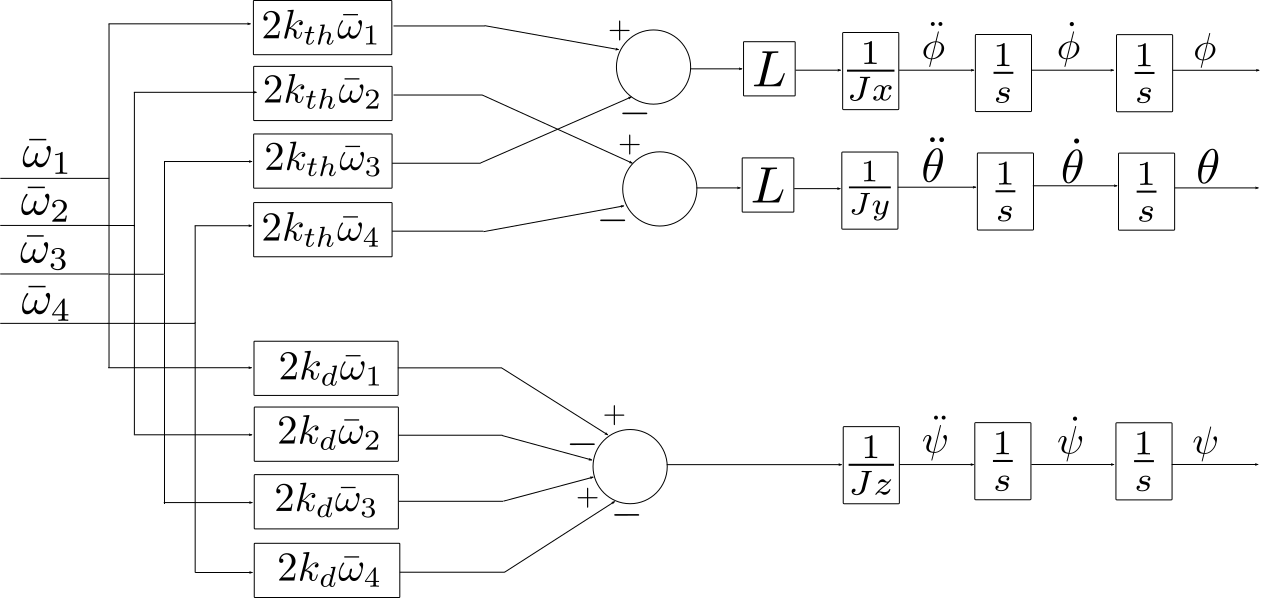
\includegraphics[scale=0.45]{figures/LinearModelBlockDiagram.pdf}
	\caption{.}
	\label{fig:LinearModelBlockDiagram}
\end{figure}

\subsection{Simulation}
The simulation of the model is done in Simulink. The parameters used for the simulations are shown in \autoref{ParametersQuadcopter}.
\begin{table}[H]
	\centering
	\begin{tabular}{|l|l|l|p{3cm}|}
		\hline %-----------------------------------------------------------------------------------
		\textbf{Parameter Name}&\textbf{Symbol} &\textbf{Value} &\textbf{Units}\\
		\hline %-----------------------------------------------------------------------------------
		Mass of the quadcopter  & $m$ & 0.996       &kg\\
		\hline
		%-----------------------------------------------------------------------------------
		Moment of inertia around x axis       & $J_x$  & 0.01073       & $kg \cdot m^2$\\
		\hline %-----------------------------------------------------------------------------------
		Moment of inertia around y axis       & $J_y$  & 0.01073       & $kg \cdot m^2$\\
		\hline %-----------------------------------------------------------------------------------
		Moment of inertia around z axis       & $J_z$  & 0.02135       & $kg \cdot m^2$\\
		\hline %-----------------------------------------------------------------------------------
		Length of quadcopter rm       & $L$  &   0.225       & $m$\\
		\hline %-----------------------------------------------------------------------------------
		Thrust force constant       & $k_{th}$  & -       & $kg \cdot m^2$\\
		\hline %-----------------------------------------------------------------------------------\\
		Drag torque constant      & $k_{d}$  & -       & $kg \cdot m^2$\\
		\hline %-----------------------------------------------------------------------------------\\
	\end{tabular}
	\caption{Parameters used in the simulation of the model.}
	\label{ParametersQuadcopter}
\end{table}\vspace{-18pt}

\subsubsection{Attitude Model Simulations}
In \autoref{fig:rollCompModel}, \ref{fig:pitchCompModel} and \ref{fig:yawCompModel}, the angular behavior of the model around the is analyzed. The input to the system are the four motor velocities. They are defined so the response of the model is predictable and the its performance can be evaluated.

The behavior around x axis is shown in \autoref{fig:rollCompModel}. Only the speeds of motors 2 and 4 are changed as they are supposed to be the ones that affect the roll angle. It can be seen that a positive difference in the rotation speed of these motors generates a positive acceleration in the roll direction, which is consistent with \autoref{eq:AngleEqVelocitiescombined1}.

It can also be observed that the linear approximation of the equations yields an accurate result as the two responses show no perceptible difference. 
%
\begin{figure}[H]
	\centering
	\includegraphics[scale=0.65]{figures/rollCompModel}
	\caption{.}
	\label{fig:rollCompModel}
\end{figure}
%
The behavior around the y axis is very similar to that of the roll angle. It is shown in \autoref{fig:pitchModel}. In this case, the motor velocities that are modified are those from motors 1 and 3. 
%
\autoref{eq:AngleEqVelocitiescombined2} states that a positive rotational speed difference creates a positive pitch acceleration. This is confirmed by the simulations in both models. Again, the linear approximation can be considered adequate.
\begin{figure}[H]
	\centering
	\includegraphics[scale=0.65]{figures/pitchCompModel}
	\caption{.}
	\label{fig:pitchCompModel}
\end{figure}
%

%
\begin{figure}[H]
	\centering
	\includegraphics[scale=0.65]{figures/yawCompModel}
	\caption{.}
	\label{fig:yawCompModel}
\end{figure}
\fxnote{Title should say z-axis}

\subsubsection{Translational Model Simulations}
\begin{figure}[H]
	\centering
	\includegraphics[scale=0.65]{figures/xCompModel}
	\caption{.}
	\label{fig:xCompModel}
\end{figure}

\begin{figure}[H]
	\centering
	\includegraphics[scale=0.65]{figures/yCompModel}
	\caption{.}
	\label{fig:yCompModel}
\end{figure}

\begin{figure}[H]
	\centering
	\includegraphics[scale=0.65]{figures/zCompModel}
	\caption{.}
	\label{fig:zCompModel}
\end{figure}

	
	%%% Part 2 %%%
	\part{Design and Implementation}
	%---------- Chapter 5 -----------------------------------------------------------
	\chapter{Network} \label{ch:Network}

%The control of a quadcopter implies, in most cases, the use of a wireless network.
As mentioned in \autoref{sec:PrototypeDescription} the quadcopter relies on a network between the ground station and the microcontroller. The information transmitted to the microcontroller is the attitude, position, translational velocity and the position reference.

%The control of such a system through a network requires the 
To ensure that the microcontroller can detect packets and disregard incorrect packets received from the computer, a protocol is necessary. As mentioned in \autoref{sec:hardware} the lower level communication is handled by the Xbees, and therefore only the transport layer is designed.

%design of a communication protocol. The use of the XBEE modules makes the design easier as only the transport layer must be taken into account. 
%As typical for real time systems, this will be a connectionless protocol to ensure the data transmission is as fast as possible.

The effects of the network in the control system are analyzed using the Matlab toolbox, TrueTime. The issues considered are the delay from the sensor to the controller and the missed packets. Missed packets are considered to be when the controllers does not utilize the data from a new received packet, for any reason, in each loop. These issues are taken into account as they disturb the control system the most.
%The Vicon system has a sampling rate of 100 Hz. A connectionless protocol can thereby be utilized, as it is sufficient to transmit the latest data to the microcontroller instead of asking for a retransmission, e.g. if a packet is lost or corrupt. Furthermore a retransmission will cause a delay in the system, this is not desired as this real time system is sensitive to delay.
	\section{Communication Protocol}

Explain the communication protocol
	\section{Delay}
The delay in the system constitutes one of the main network effects in the system. It forces the controller design to be more robust and that means in most cases to make them slower. In order to consider the delay in the controller design, the TrueTime simulation toolbox for MATLAB is utilized. This toolbox allows to simulate the control design, the derived model and the wireless network together in order to find a control design that is still stable.

In the simulation, a model for the delay needs to be found in order to implement it in TrueTime. The chosen approach is to model the delay as the maximum possible delay appearing in the system so the worst case scenario is considered. Its value has been obtained by adding the time required to make the information available in the microcontroller and the maximum time elapsed since the data is available until it is used by the microcontroller. 

The time required to make the data available can be divided into three. The time required to send the data, the transmission delay and the time it takes to decode the information in the microcontroller. The first and the third of these, can be found exactly as it is code execution time, the values obtained are 15 and 7.64 ms respectively. The transmission time can be found using the transmission speed of the Xbee modules. According to the datasheet \fxnote{source datasheet}, this is  115,2 kbit/s. With this speed and taking into account 21 bytes are transmitted, the transmission delay is 1.46 ms.

Once the information is on the microcontroller, the maximum time elapsed until the controller uses it is the sampling time minus the time needed to decode a package minus the execution time of the control loop. This is so because in the worst possible case, the package arrives just after the previous control loop finishes, then it is necessary to wait until the information is processed and until the next control loop is executed. 

\autoref{fig:delaycontrol} shows the different networked induced delays in the system and the maximum delay. 
\begin{figure}[H]
	\centering
	\includegraphics[width=.6\textwidth]{figures/maxDelay.pdf}
	\caption{Delays in the packages transmitted to the microcontroller and maximum delay.\fxnote{Check times when we have them all}}
	\label{fig:delaycontrol}
\end{figure}

After all considerations, the value of the delay used in the simulation is 50.6 ms\fxnote{Check delay when we have them all}.

%since the information is obtained until it is sent through the network, the transmission delay and the time needed to process the information in the microcontroller. being exponentially distributed. \autoref{eq:exponentialdist} shows the probability and cumulative density functions of the exponential distribution.
%\begin{flalign}
%		f=-\lambda\mathrm{e}^{-\lambda t}\mathrm{;}\ \ \ \ \  F=1-\mathrm{e}^{-\lambda t}
%		\label{eq:exponentialdist}
%\end{flalign}
%\begin{where}
%	\va{f} {is the probability density function} { }
%	\va{F} {is the cumulative density function} { }
%	\va{\lambda} {is the rate parameter} { }
%	\va{t} {is time} { }
%\end{where}
%The parameter lambda can be interpreted as the inverse of the mean time between observations, that is, the mean delay in the system. The value for this parameter has been found experimentally by measuring and averaging the experienced delays in \fxnote{PUT NUMBER} transmissions. The detailed experiments can be seen in \fxnote{APPENDIX WITH DATA}. The average delay obtained is \fxnote{PUT NUMBER} which leads to a value for $\lambda$ of \fxnote{PUT NUMBER}
 
%To generate the exponential distributed delays, the inverse transformation theorem has been applied. This theorem allows to transform an uniformly distributed random variable, easier to generate, into a random variable distributed with any other known cumulative density function. \autoref{eq:invtransthorem} illustrates this theorem.
%\begin{flalign}
%	\mathrm{Y}= F^{-1}\mathrm{X}
%	\label{eq:invtransthorem}
%\end{flalign}
%\begin{where}
%	\va{F} {is the desired cumulative density function for the random variable} { }
%	\va{\mathrm{X}} {is a uniformly distributed random variable} {}
%	\va{\mathrm{Y}} {is a random variable distributed according to the cumulative density function $F$} {}
%\end{where}

%The final expression obtained can be seen in \autoref{eq:formuladelay}.
%\begin{flalign}
%	\mathrm{delay}= -\frac{\ln(1-\mathrm{X})}{\lambda}
%	\label{eq:formuladelay}
%\end{flalign}







	
	%---------- Chapter 6 ----------------------------------------------------------- 	
	\chapter{Controller Design}\label{chap:Control}

Control Strategy (all the relations between controllers)\\
Flow of chapter\\	
	\subsection{Attitude Controller}
The attitude controller for the quadcopter has been designed using a state space representation of the system. This helps handling the coupled angular response of the quadcopter. The chosen states for the system are the three angular positions and the three angular velocities. The input vector of the attitude system consists of the four motor rotational speeds and the output vector consists of the three angles, roll, pitch and yaw. Below, the state, input and the output vectors are presented.
%
\begin{flalign}
	\vec{x}(t) = 
	\begin{bmatrix}
		\phi & \theta & \psi & \dot{\phi} &	\dot{\theta} & \dot{\psi} \\
	\end{bmatrix}	\nonumber
	^T
	\label{xVector}
\end{flalign}  
\begin{flalign}
	\vec{y}(t) = 
	\begin{bmatrix}
		\phi &	\theta & \psi \\
	\end{bmatrix}	\nonumber
	^T
	\label{yVector}
\end{flalign}
\begin{flalign}
	\vec{u}(t)= 
	\begin{bmatrix}
		\omega_1 & \omega_2 &	\omega_3 &	\omega_4 \\
	\end{bmatrix}\nonumber	
	^T
	\label{uVector}+
\end{flalign}
%
The above is then used in construction of the state space matrix representation as displayed in \autoref{xDotSS} and \ref{ySS}.
\begin{flalign}
	\vec{\dot{x}}(t)&=\vec{A} \cdot \vec{x}(t) + \vec{B} \cdot \vec{u}(t)
	\label{xDotSS} 
\end{flalign}
\begin{flalign}
	\vec{y}(t)&=\vec{C} \cdot \vec{x}(t) + \vec{D} \cdot \vec{u}(t)\label{ySS} 
\end{flalign}

Where $\vec{A}$ is the system matrix, $\vec{B}$ is the input matrix, $\vec{C}$ is the output matrix and $\vec{D}$ is the feedback matrix.

The values for the $\vec{A}$, $\vec{B}$, $\vec{C}$ and $\vec{D}$ matrices are obtained from the linearized attitude equations, yielding the matrices shown below. As $\vec{D}$ is a zero matrix, only $\vec{A}$, $\vec{B}$ and $\vec{C}$ are shown. 
\footnotesize
\begin{flalign}   \label{Amatrix}
	\vec{A}=
	\begin{bmatrix}
		\ 0 & 0 & 0 & 1 & 0 & 0     \ \ \ \\ 
		\ 0 & 0 & 0 & 0 & 1 & 0     \ \ \ \\ 
		\ 0 & 0 & 0 & 0 & 0 & 1     \ \ \ \\
		\ 0 & 0 & 0 & 0 & 0 & 0     \ \ \ \\ 
		\ 0 & 0 & 0 & 0 & 0 & 0     \ \ \ \\ 
		\ 0 & 0 & 0 & 0 & 0 & 0     \ \ \  		
	\end{bmatrix}\nonumber
\end{flalign} \label{Bmatrix}
\begin{flalign}
    \vec{B} =
	\begin{bmatrix}
		\ 0 & 0 & 0 & 0      \ \ \ \\ 
		\ 0 & 0 & 0 & 0      \ \ \ \\ 
		\ 0 & 0 & 0 & 0      \ \ \ \\
		\ 0 & \si{-\frac{2 \cdot k_{th} \cdot L \cdot \overline{\omega}_2}{J_x}} & 0 & \si{\frac{2 \cdot k_{th} \cdot L \cdot \overline{\omega}_4}{J_x}}      \ \ \ \\ 
		\ \si{\frac{2 \cdot k_{th} \cdot L \cdot \overline{\omega}_1}{J_y}} & 0 & \si{-\frac{2 \cdot k_{th} \cdot L \cdot \overline{\omega}_3}{J_y}} & 0      \ \ \ \\ 
		\ \frac{2 \cdot k_d \cdot {\overline{\omega}_1}}{J_z} & - \frac{2 \cdot k_d \cdot {\overline{\omega}_2}}{J_z} & \frac{2 \cdot k_d \cdot {\overline{\omega}_3}}{J_z} & - \frac{2 \cdot k_d \cdot {\overline{\omega}_4}}{J_z}      \ \ \ 		
	\end{bmatrix}\nonumber
\end{flalign}
\begin{flalign} \label{Cmatrix}
	\vec{C} =	 
	\begin{bmatrix}
		\ 1 & 0 & 0 & 0 & 0 & 0     \ \ \ \\ 
		\ 0 & 1 & 0 & 0 & 0 & 0     \ \ \ \\ 
		\ 0 & 0 & 1 & 0 & 0 & 0     \ \ \ 		
	\end{bmatrix}\nonumber
\end{flalign}
\normalsize

This system can also be proven to be both controllable and observable, which are necessary conditions to be able to design a observer-based control.

For the quadcopter to hover, it is desired to keep the attitude in equilibrium; this is achieved using a state feedback. To be able to change and track a reference an integral controller is designed combined with the other one. It is also desirable to use an observer in order to estimate the angular velocities that are part of the state of the system. This is done using a reduced-order observer. These two designs can be done independently due to the separation principle. \cite{ssReference}

\autoref{AttitudeControlDiagram} shows how this designs are related.

\begin{figure}[H]
    \centering
    \includegraphics[scale=0.3]{figures/AttitudeControlDiagram}
    \caption{ Control structure for the system, including the state feedback, the integral control and the reduced order observer.}
    \label{AttitudeControlDiagram}
\end{figure}

%--------------------- StateFeedback with Integral Control ----------------------------
The control design is shown in \autoref{fig:DetailedControllerColorDiagram}.
\begin{figure}[H]
    \includegraphics[scale=.35]{figures/DetailedControllerColorDiagram}
    \centering
    \captionof{figure}{Detail of the left diagram, that includes all the variables used in the design of the controller.}
    \label{fig:DetailedControllerColorDiagram}
\end{figure}

It can be seen that there are three new states that are added to the system, $\vec{x}_{Int}(t)$ and lead to the extended system shown in \autoref{xdotSSExtended} and \ref{ySSExtended}.
%
\begin{flalign} 
\dot{\vec{x}}_e(t) &= \vec{A}_e \  \vec{x}_e(t) + \vec{B}_e \  \vec{u}(t) + 
\begin{bmatrix}
\ \vec{0}     \ \ \ \\ 
\ \vec{-I}     \ \ \  		
\end{bmatrix}
\vec{r}(t) 
\label{xdotSSExtended}\\ 
\vec{y}(t) &= \vec{C}_e \  \vec{x}_e 
\label{ySSExtended}
\end{flalign} 
%
being\\
\scriptsize
\begin{minipage}{0.28\linewidth}
    \begin{flalign}
    \dot{\vec{x}}_e(t)= 
    \begin{bmatrix}
    \ \dot{\vec{x}}(t)      \ \  \\ 
    \ \dot{\vec{x}}_{Int}(t)      \ \   		
    \end{bmatrix} \nonumber
    \end{flalign}
\end{minipage}\hfill
\begin{minipage}{0.2\linewidth}
    \begin{flalign}
    \vec{A}_e=
    \begin{bmatrix}
    \ \vec{A}  & \vec{0}    \ \  \\ 
    \ \vec{C}  & \vec{0}    \ \   		
    \end{bmatrix} \nonumber
    \end{flalign}
\end{minipage}   \hfill 
\begin{minipage}{0.2\linewidth}
    \begin{flalign}
    \vec{B}_e=
    \begin{bmatrix}
    \ \vec{B}    \ \  \\ 
    \ \vec{0}     \ \   		
    \end{bmatrix} \nonumber
    \end{flalign}
\end{minipage}\hfill
\begin{minipage}{0.2\linewidth}
    \begin{flalign}
    \vec{C}_e=
    \begin{bmatrix}
    \ \vec{C}  & \vec{0}  \ \   		
    \end{bmatrix} \nonumber
    \end{flalign}
\end{minipage}
\normalsize
\\

With this approach, the control law given by \autoref{eq:ssControllerAction}.
%
\begin{flalign} 
    \vec{u}(t) &=\vec{F} \  \vec{x}(t) + \ \vec{F}_{Int} \  \vec{x}_{Int}(t)
    \label{eq:ssControllerAction}
\end{flalign}
%
The resulting feedback law can be design as a conventional state feedback, where the goal is to choose an appropriate $F_e=[F \ F_{Int}]$ matrix such that the eigenvalues of $A_e+B_eF_e$ are the new poles that the system needs to have in order to achieve the desired dynamics.

Once $F_e$ is obtained, it can be split into $F$ and $F_{Int}$ by taking the first 6 columns for the state feedback and the last 3 for the integral control. In this way, the controller can be implemented as shown in \autoref{fig:DetailedControllerColorDiagram}.

%--------------------- Reduced-Order Observer ----------------------------


In general an observer is utilized in a control system if either one of two specific cases occurs. If certain states in the system are not measured, an observer can estimate the unmeasured states by means of the system output and input. However, it is also possible to use an observer if the measured data gathered from the sensors is affected by noise. The observer can thereby use both the noisy measured states and the estimated states creating a filtered version. This case will however not be utilized in the prototype.

With this approach, the first three states, $x_1$ with be equal to the outputs, $y$, whereas the other three states will be estimated, $\hat{x}_2$.

The matrices that define the original system can be split into submatrices, that will be used in the design of the observer, as follows:\\
%
\begin{minipage}{0.45\linewidth}
    \begin{flalign}
    \vec{A}=
    \begin{bmatrix}
    \ \vec{A11}_{3 \times 3}  & \vec{A12}_{3 \times 3}    \ \ \ \\ 
    \ \vec{A21}_{3 \times 3}  & \vec{A22}_{3 \times 3}    \ \ \  		
    \end{bmatrix} \nonumber
    \end{flalign}
\end{minipage}   \hfill 
\begin{minipage}{0.45\linewidth}
    \begin{flalign}
    \vec{B}=
    \begin{bmatrix}
    \ \vec{B1}_{3 \times 4}    \ \ \ \\ 
    \ \vec{B2}_{3 \times 4}     \ \ \  		
    \end{bmatrix} \nonumber
    \end{flalign}
\end{minipage}\hfill
\\

As described in ?? the system is observable, making it possible to find an observer gain, $L_{obs}$, which makes \autoref{eq:observerStable} stable \cite{ssReference}.
%
\begin{flalign}
    \vec{A_{22}} + \vec{L_{obs}}\vec{A_{A12}} \label{eq:observerStable}
\end{flalign}

With this observer gain, the observer in \autoref{eq:observerStable} ensures an estimate $\hat{x}_2$ which converges to $x_2$ at a rate given by the eigenvalues of \autoref{eq:eqobservertheorem}.
\small
\begin{flalign}
    \vec{\hat{\dot{x}}_2} &= \vec{A_{21}}\vec{y} + \vec{A_{22}}\vec{\hat{x}_2} + \vec{B_2u} + \vec{L_{obs}}\vec{(A_{12}\hat{x}_2} - \vec{A_{21}x_2}) \label{eq:eqobservertheorem}
\end{flalign}
\normalsize \\
This estimation of $\hat{x}_2$ can also be seen\autoref{fig:observerDiagram}.
\begin{figure}[H]
    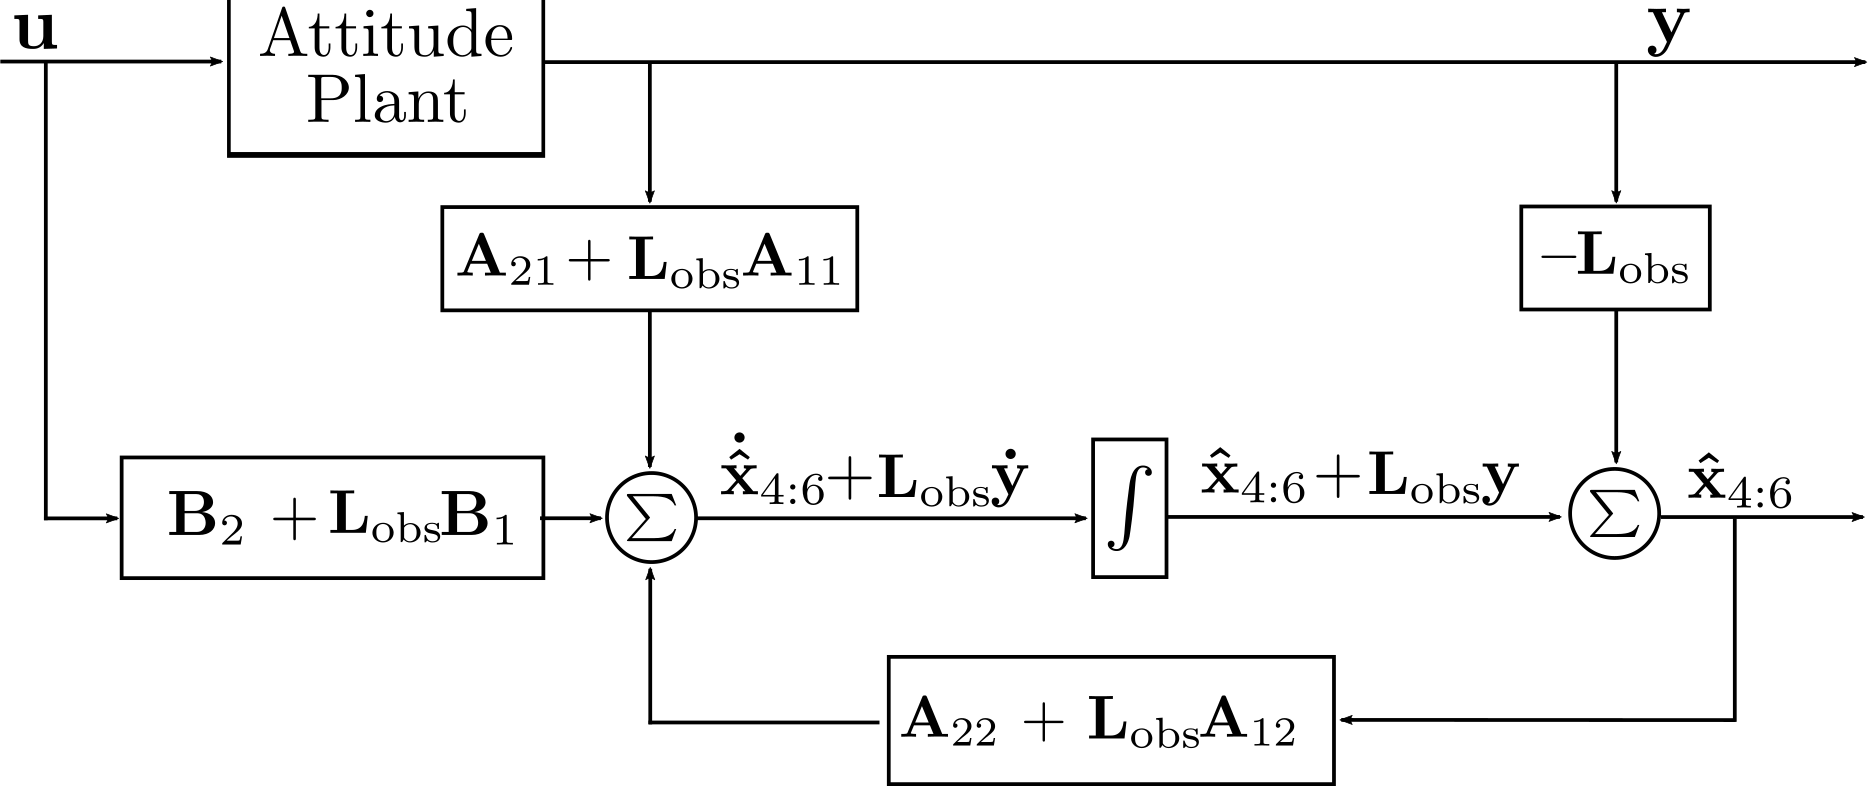
\includegraphics[scale=.2]{figures/observerDiagram}
    \centering
    \captionsetup{justification=centering}
    \captionof{figure}{This diagram should be made so it looks a bit more similar to the previous on. But only the part with the observer.}
    \label{fig:observerDiagram}
\end{figure}












	\subsection{State Feedback with Integral Control Design}
The aim of the controller is to be able to track a reference in the three angles that define the attitude of the quadcopter.

Given a state space representation as the one in \autoref{xDotLinear} and \ref{yLinear}, it is possible to design a controller so that the final dynamics of the system can be chosen.

In this approach a state feedback is used to allow the system to return to equilibrium position while an integral controller makes it possible to include a reference and track it, adding both control actions to get the one finally applied to the motors. The diagram in \autoref{fig:DetailedControllerColorDiagram} shows how these controllers are related.
%
\begin{minipage}{\linewidth}
	\begin{minipage}{0.6\linewidth}
		\begin{figure}[H]
			\includegraphics[scale=.35]{figures/ControllerColorDiagram}
			\centering			
			\captionof{figure}{Control structure with the state feedback and integral control parts highlighted.}
			\label{fig:ControllerColorDiagram}
		\end{figure}
	\end{minipage}
	\hspace{0.03\linewidth}
	\begin{minipage}{0.4\linewidth}
		\begin{figure}[H]\vspace{20mm}
			\includegraphics[scale=.35]{figures/DetailedControllerColorDiagram}
			\centering \vspace{7mm}
			\captionof{figure}{Detail of the left diagram, that includes all the variables used in the design of the controller.}
			\label{fig:DetailedControllerColorDiagram}
		\end{figure}
	\end{minipage}
\end{minipage}


From \autoref{fig:DetailedControllerColorDiagram}, the feedback law yields \autoref{eq:ssControllerAction}.
%
\begin{flalign} 
	\vec{u}(t) &=\vec{F} \  \vec{x}(t) + \ \vec{F}_{Int} \  \vec{x}_{Int}(t)
     \label{eq:ssControllerAction}
\end{flalign}
%
\begin{where}
	\va{\vec{F}}{is the 4x6 state feedback matrix}{}
	\va{\vec{F}_{Int}}{is the 3x6 integral feedback matrix }{}
\end{where}

In this equation, \si{\vec{x}_{Int}(t)} is given by \autoref{eq:ssControllerAction1}, that is equivalent to \autoref{eq:ssControllerAction2}, see \autoref{fig:DetailedControllerColorDiagram}.
\begin{flalign}
    \vec{x}_{Int}(t) &= \int_{0}^{t} \vec{y}(\tau)-\vec{r}(\tau) d\tau	\label{eq:ssControllerAction1}\\
    \vec{\dot{x}}_{Int}(t) &= \vec{y}(t)-\vec{r}(t) \label{eq:ssControllerAction2}
\end{flalign} 
%
This last equation can be introduced in the existing state space model, taking \si{\vec{x}_{Int}(t)} as new states, and giving the result shown in \autoref{xdotSSExtended} and \autoref{ySSExtended}.
%
\begin{flalign} 
    \dot{\vec{x}}_e(t) &= \vec{A}_e \  \vec{x}_e(t) + \vec{B}_e \  \vec{u}(t) + 
    \begin{bmatrix}
       \ \vec{0}     \ \ \ \\ 
       \ \vec{-I}     \ \ \  		
   \end{bmatrix}
   \vec{r}(t) 
   \label{xdotSSExtended}\\ 
    \vec{y}(t) &= \vec{C}_e \  \vec{x}_e 
       \label{ySSExtended}
\end{flalign} 
%
being\\
\begin{minipage}{0.24\linewidth}
	\begin{flalign}
		\dot{\vec{x}}_e(t)= 
		\begin{bmatrix}
			\ \dot{\vec{x}}(t)      \ \ \ \\ 
			\ \dot{\vec{x}}_{Int}(t)      \ \ \  		
		\end{bmatrix} \nonumber
	\end{flalign}
\end{minipage}\hfill
\begin{minipage}{0.24\linewidth}
	\begin{flalign}
	    \vec{A}_e=
	    \begin{bmatrix}
	        \ \vec{A}  & \vec{0}    \ \ \ \\ 
	        \ \vec{C}  & \vec{0}    \ \ \  		
	    \end{bmatrix} \nonumber
	\end{flalign}
\end{minipage}   \hfill 
\begin{minipage}{0.24\linewidth}
	\begin{flalign}
		\vec{B}_e=
		\begin{bmatrix}
			\ \vec{B}    \ \ \ \\ 
			\ \vec{0}     \ \ \  		
		\end{bmatrix} \nonumber
	\end{flalign}
\end{minipage}\hfill
\begin{minipage}{0.24\linewidth}
	\begin{flalign}
		\vec{C}_e=
		\begin{bmatrix}
			\ \vec{C}  & \vec{0}  \ \ \  		
		\end{bmatrix} \nonumber
	\end{flalign}
\end{minipage}

The resulting feedback law can be design as a conventional state feedback, where the goal is to choose an appropriate $\vec{F}_e=[\vec{F} \ \vec{F}_{Int}]$ matrix such that the eigenvalues of $\vec{A}_e+\vec{B}_e\vec{F}_e$ are the new poles that the system needs to have in order to achieve the desired dynamics. The poles are chosen such that the system is as fast as possible taking into account also the network induced effects described in \autoref{ch:Network}. The poles are placed in $[-3, -3.2, -3.3, -3.4, -3.5, -3.6, -3.7, -3.8, -3.9]$.

Once $\vec{F}_e$ is obtained, it can be split into $\vec{F}$ and $\vec{F}_{Int}$ by taking the first 6 columns for the state feedback and the last 3 for the integral control. These matrices can be sen in \autoref{app:matricesSS}. In this way, the controller can be implemented as shown in \autoref{fig:DetailedControllerColorDiagram}.


 			  %----- Subsection
	
It is decided to implement a linear quadratic regulator (LQR) as it is necessary to priorities the different states and ensure that the control action does not exceed its limits. This can be done by minimizing \autoref{eq:costfunction}.

\begin{flalign} 
	J &= \int_{0}^{\infty} \vec{x}^T \vec{Q} \vec{x} + \vec{u}^T \vec{R} \vec{u} \ dt\\
     \label{eq:costfunction}
\end{flalign}
\begin{where}
	\va{\vec{Q}}{is a positive semi-definite diagonal matrix}{}
	\va{\vec{R}}{is a positive definite diagonal matrix}{}
	\va{\vec{J}}{is a scalar}{}
\end{where}

This cost function contains weighting factors, the $\vec{Q}$ and $\vec{R}$ matrices. The weighting factors are used to either penalize or priorities different states and inputs. When weighting the states, it is possible to give the yaw more gain than the roll and pitch if necessary. By weighting the inputs, it is possible to ensure that they do not yield a control action which exceeds its limits. The $\vec{Q}$ matrix is semi-definite as the weighted states, $\vec{x}^T\vec{Q}\vec{x}$, has the possibility of becoming zero even though the states are above zero??? The $\vec{R}$ matrix is positive definite as an control action is always desired??? By minimize the cost function J, it is possible to regulate the $\vec{x}$ to zero as time goes to infinity??

To design a state feedback which minimize \autoref{eq:costfunction} the optimal state feedback law stated in \autoref{eq:optimalstatefeedbacklaw} is utilized.

\begin{flalign} 
	\vec{u} &= \vec{F}\vec{x}\\
     \label{eq:optimalstatefeedbacklaw}
\end{flalign}

where $\vec{F}$ is:

\begin{flalign} 
	\vec{F} &= -\vec{R}^{-1}\vec{B}^T\vec{P}\\
     \label{eq:optimalF}
\end{flalign}
\begin{where}
	\va{\vec{P}}{is }{}
\end{where}

And $\vec{P}$ can be found from:

\begin{flalign} 
	\vec{A}^T\vec{P}+\vec{P}\vec{A}-\vec{P}\vec{B}\vec{R}^{-1}\vec{B}^T\vec{P}+\vec{Q} &= \vec{0}\\
     \label{eq:optimalP}
\end{flalign}

To find the $\vec{Q}$ and $\vec{R}$ matrices Bryson's rule is utilized:
Bryson's rule:

\begin{flalign} 
	Q_{ii} &= \frac{1}{\text{maximum acceptable value of }[x^2_i]}\\
	R_{ii} &= \frac{1}{\text{maximum acceptable value of }[u^2_i]}
     \label{eq:weightingmatrices}
\end{flalign}

The weighting matrices, $\vec{Q}$ and $\vec{R}$, can the be found through iterations, and a compromise between desired performance and control action can be found. 
 
	\subsection{Reduced Order Observer}
It has been decided to implement a reduced order observer, to observer the angular velocities. In general an observer is utilized in a control system if either one of two specific cases occurs. If certain states in the system are not measured, an observer can estimate the unmeasured states by the means of some of the measured state-variables. However, it is also possible to use an observer if the measured data gathered from the sensors is affected a significant amount of noise. As the observer in addition to estimating unmeasured states, also filters measurements \fxnote{feedback control of dynamic systems page 515}. The latter is however not focus more on in the prototype.

As explained earlier, the attitude model has six states, the three angles of the quadcopter (roll, pitch and yaw) and the three angular velocities. By using the Vicon system, the three angles of the quadcopter are measured, making it possible to estimate the angular velocities. With this approach, the first three states (angles), $x_1$ will be equal to the outputs, $y$, whereas the other three states will be estimated (angular velocities), $\hat{x}_2$.

In \autoref{fig:Observerdiagram1} a diagram illustrating the setup of the angular controller is shown. The highlighted lines is the reduced order observer and its corresponding inputs and output.
%
\begin{figure}[H]
    \includegraphics[scale=.4]{figures/ObserverColorDiagram}
    \centering			
    \captionof{figure}{An overall block diagram of the angular controller highlighting the reduced order observer and its corresponding inputs and output.}
    \label{fig:Observerdiagram1}
\end{figure}
%
The matrices which define the system can be separated into submatrices, which will be used in the design of the observer:\\
%
\begin{minipage}{0.45\linewidth}
    \begin{flalign}
        \vec{A}=
        \begin{bmatrix}
            \ \vec{A11}_{3 \times 3}  & \vec{A12}_{3 \times 3}    \ \ \ \\ 
            \ \vec{A21}_{3 \times 3}  & \vec{A22}_{3 \times 3}    \ \ \  		
        \end{bmatrix} \nonumber
    \end{flalign}
\end{minipage}   \hfill 
\begin{minipage}{0.45\linewidth}
    \begin{flalign}
        \vec{B}=
        \begin{bmatrix}
            \ \vec{B1}_{3 \times 4}    \ \ \ \\ 
            \ \vec{B2}_{3 \times 4}     \ \ \  		
        \end{bmatrix} \nonumber
    \end{flalign}
\end{minipage}\hfill
%\begin{minipage}{0.33\linewidth}
%    \begin{flalign}
%        \vec{C}=
%        \begin{bmatrix}
%            \ \vec{C}_{3 \times 3}  & \vec{0}_{3 \times 3}  \ \ \  		
%        \end{bmatrix} \nonumber
%    \end{flalign}
%\end{minipage}


As described before the system is observable. It is thereby possible to utilize the reduced order observer theorem \fxnote{The reduced order observer theorem slide 6 course 4 control.}. This theorem states, that for an observable system there always exist an gain $L_{obs}$ which ensures that \autoref{eq:observerStable} is stable.
%
\begin{flalign}
	\vec{A_{22}} + \vec{L_{obs}}\vec{A_{12}}
		\label{eq:observerStable}
\end{flalign}
%
The theorem also states that with this observer gain, the observer in \autoref{eq:eqobservertheorem} ensures that the estimate, $\hat{x}_2$, converges to $x_2$ with a rate yielded by the eigenvalues of \autoref{eq:eqobservertheorem}.
%
\begin{flalign}
	\vec{\hat{\dot{x}}_2} &= \vec{A_{21}}\vec{y} + \vec{A_{22}}\vec{\hat{x}_2} + \vec{B_2u} + \vec{L_{obs}}\vec{(A_{12}\hat{x}_2} - \vec{A_{21}x_2})
		\label{eq:eqobservertheorem}
\end{flalign}
%
To calculate an appropriate observer gain, $L_{obs}$, it is necessary to evaluate the reliability of the utilized sensor. If the gain is set very high, the estimation will rely more on the actual measurements of the outputs, whereas if it is very low, there will be more influence of the model in the final calculations \fxnote{christoffer slide 35 course 3}.

%The matrix in \autoref{Matrix:Lobs} is the decided observer gains utilized in the reduced order observer.
%
%\begin{flalign}
%	\vec{L_{obs}} = 
%	\begin{bmatrix}
%	\ -50 & 0 & 0  \ \ \ \\ 
%	\ 0 & -60 & 0  \ \ \ \\ 
%	\ 0 & 0 & -70  \ \ \  
%	\end{bmatrix}
%	\label{Matrix:Lobs}
%\end{flalign}

With the final design, \autoref{eq:eqobserverderived} shows how to estimate $\hat{x}_2$.
%
\begin{flalign}
    \vec{\hat{\dot{x}}_2} + \vec{L\dot{y}} &= \vec{(A_{22}} + \vec{LA_{12})\hat{x}_2} + \vec{(A_{21}} + \vec{LA_{11})y} + (\vec{B_2} + \vec{LB_1})\vec{u}
    \label{eq:eqobserverderived}
\end{flalign}
%
This estimation can also be seen in the form of a block diagram, \autoref{fig:observerDiagram}.
\begin{figure}[H]
	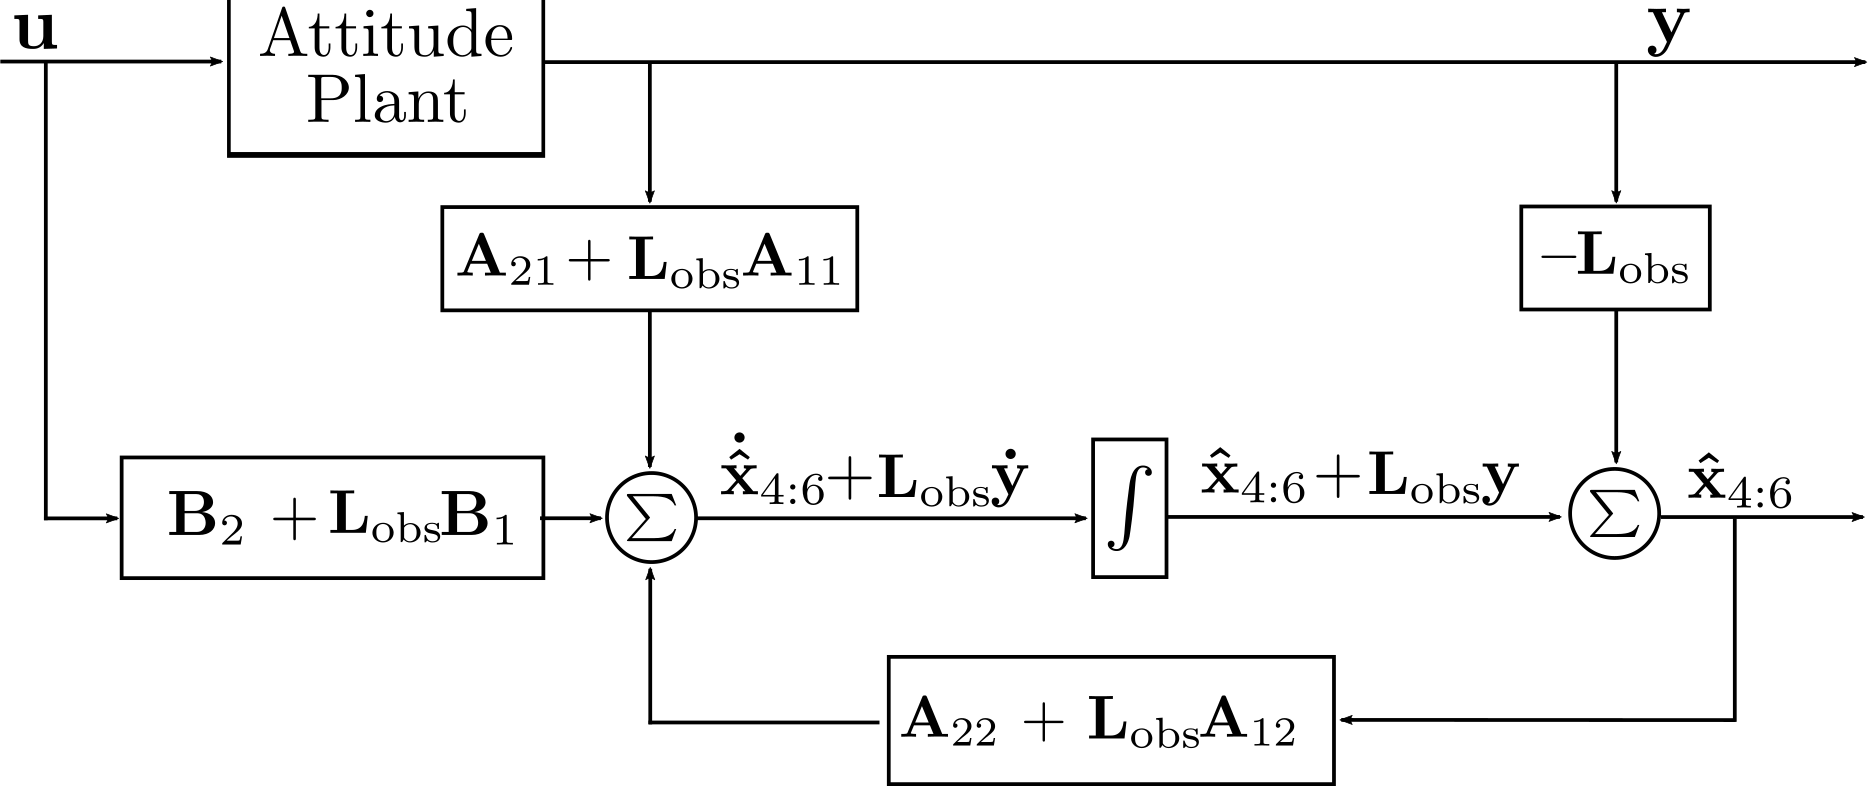
\includegraphics[scale=.35]{figures/observerDiagram}
	\centering
	\captionsetup{justification=centering}
	\captionof{figure}{A diagram showing the reduced order observer and how it is implemented.}
	\label{fig:observerDiagram}
\end{figure}











%\begin{minipage}{0.15\linewidth}
%	\begin{flalign}
%	A_{11} = 
%	\begin{bmatrix}
%		\ 0 & 0 & 0 \ \ \\ 
%		\ 0 & 0 & 0 \ \ \\ 
%		\ 0 & 0 & 0 \ \ \\
%	\end{bmatrix}	\nonumber
%	\label{A11}
%	\end{flalign}  
%\end{minipage}\hfill
%\begin{minipage}{0.15\linewidth}
%	\begin{flalign}
%	A_{12} = 
%	\begin{bmatrix}
%		\ 1 & 0 & 0 \ \ \\ 
%		\ 0 & 1 & 0 \ \ \\ 
%		\ 0 & 0 & 1 \ \ \\
%	\end{bmatrix}	\nonumber
%	\label{A12}
%	\end{flalign}
%\end{minipage}\hfill
%\begin{minipage}{0.15\linewidth}
%	\begin{flalign}
%	A_{21} = 
%	\begin{bmatrix}
%		\ 0 & 0 & 0 \ \ \\ 
%		\ 0 & 0 & 0 \ \ \\ 
%		\ 0 & 0 & 0 \ \ \\
%	\end{bmatrix}	\nonumber
%	\label{A21}
%	\end{flalign}
%\end{minipage}\hfill
%\begin{minipage}{0.15\linewidth}
%	\begin{flalign}
%	A_{22} = 
%	\begin{bmatrix}
%		\ 0 & 0 & 0 & 0 \ \ \\ 
%		\ 0 & 0 & 0 & 0 \ \ \\ 
%		\ 0 & 0 & 0 & 0 \ \ \\
%	\end{bmatrix} \nonumber
%	\label{A22}
%	\end{flalign}
%\end{minipage}\hfill
%
%
%\begin{minipage}{0.4\linewidth}
%	\begin{flalign}
%	B_1 = 
%	\begin{bmatrix}
%		\ 0 & 0 & 0 & 0 \ \ \\ 
%		\ 0 & 0 & 0 & 0 \ \ \\ 
%		\ 0 & 0 & 0 & 0 \ \ \\
%	\end{bmatrix}	\nonumber
%	\label{B1}
%	\end{flalign}
%\end{minipage}\hfill
%\begin{minipage}{0.6\linewidth}
%	\begin{flalign}
%	B_2 = 
%	\begin{bmatrix}
%		0 & \si{-\frac{2 \  k_{th} \  L \  \overline{\omega}_2}{J_x}} & 0 & \si{\frac{2 \  k_{th} \  L \  \overline{\omega}_4}{J_x}} \ \ \ \\ 
%		\ \si{\frac{2 \  k_{th} \  L \  \overline{\omega}_1}{J_y}} & 0 & \si{-\frac{2 \  k_{th} \  L \  \overline{\omega}_3}{J_y}} & 0 \ \ \ \\ 
%		\frac{2 \  k_d \  {\overline{\omega}_1}}{J_z} & - \frac{2 \  k_d \  {\overline{\omega}_2}}{J_z} & \frac{2 \  k_d \  {\overline{\omega}_3}}{J_z} & - \frac{2 \  k_d \  {\overline{\omega}_4}}{J_z} \ \ \
%	\end{bmatrix} \nonumber
%	\label{B2}
%	\end{flalign}
%\end{minipage}\hfill
%
%
%\begin{flalign}
%	L_{obs} = 
%	\begin{bmatrix}
%	\ -50 & 0 & 0  \ \ \ \\ 
%	\ 0 & -60 & 0  \ \ \ \\ 
%	\ 0 & 0 & -70  \ \ \  
%	\end{bmatrix}
%	\label{Lobs}
%\end{flalign}


 				    %----- Subsection
	\subsubsection{Attitude Controller Simulation}
In the following section the final design of the attitude controller is given. Hence the final pole locations from the state feedback and the observer are provided. The final response, step response and observer estimation of the attitude controller can therefore be analysed and discussed. To be able to discussed the final result and illustrate the iteration process which has been used to find the final pole locations, the state feedback and observer are changed. Thus it is possible to yield reasoning for why the final design of the attitude controller is as it is.

A short description for the following three figures, \autoref{fig:ssFinalEq}, \autoref{fig:ssObsFinal} and \autoref{fig:ssFinalStep}, which is the final system response, step response and the estimation is given. The weighted matrices, $\vec{Q}$ and $\vec{R}$, utilized for the final attitude controller can be seen in \autoref{app:matricesSS}.

In \autoref{fig:ssFinalEq} a simulated system response of the final attitude controller is shown. Initial conditions at time zero are given to the three angles. These are set to $0.2$ radians for the pitch, $-0.3$ for the roll and $-0.2$ for the yaw. The reference which the three angles is set to converge to is zero. \\ It can be seen from the figure that it approximately takes $2.5$ seconds for the pitch and roll to settle at zero, where it only takes approximately $1.4$-$1.5$ for the yaw.

\begin{figure}[H]
	\centering
	\includegraphics[scale=0.8]{figures/ssFinalEq.pdf}
	\caption{System response of the attitude controller, with initial conditions of $0.2$ radians for the pitch, $-0.3$ radians for the roll and $-0.2$ radians for the yaw. The weighted matrices, $\vec{Q}$ and $\vec{R}$, which are utilized for the final design can be seen in \autoref{app:matricesSS}.}
	\label{fig:ssFinalEq}
\end{figure}



\begin{figure}[H]
	\centering
	\includegraphics[scale=0.7]{figures/ssObsFinal.pdf}
	\caption{\autoref{app:matricesSS}.}
	\label{fig:ssObsFinal}
\end{figure}

why are there spikes / delay. Sampling frequency 35 ms.

Final step response:

\begin{figure}[H]
	\centering
	\includegraphics[scale=0.8]{figures/ssFinalStep.pdf}
	\caption{\autoref{app:matricesSS}.}
	\label{fig:ssFinalStep}
\end{figure}

Final Observer Estimator:

steady state margin 5 percent

rise time

setling time

overshoot

The yaw because the reference is always zero, as we do not want to track the yaw.


Higher F gain:

\begin{figure}[H]
	\centering
	\includegraphics[scale=1]{figures/ssEqBad.pdf}
	\caption{\autoref{app:matricesSS}.}
	\label{fig:TranslationalControlDiagram}
\end{figure}

High Estimation L:

\begin{figure}[H]
	\centering
	\includegraphics[scale=0.8]{figures/ssObsHigh.pdf}
	\caption{\autoref{app:matricesSS}.}
	\label{fig:TranslationalControlDiagram}
\end{figure}

Response with High observer L:

\begin{figure}[H]
	\centering
	\includegraphics[scale=0.8]{figures/ssEqObsHigh.pdf}
	\caption{\autoref{app:matricesSS}.}
	\label{fig:TranslationalControlDiagram}
\end{figure}
	
	\section{Translational Controller} \label{sec:TranslationalController}

General blockdiagram with the controllers and explanation (not in high depth)

\subsection{Controllers for x and y axes}
In this section the governing model equations for the x and y axes is Laplace transformed and put on transfer function. 

For the sake of repetition, the model expression for roll and pitch are as follows:
\begin{align}
m\Delta\ddot{x}_I&= -k_{th}({\overline{\omega}_1}^2+{\overline{\omega}_2}^2+{\overline{\omega}_3}^2+{\overline{\omega}_4}^2)\cos(\overline{\theta})\Delta\theta\\ \label{eq:model_x_transl}
m\Delta\ddot{y}_I&= k_{th}({\overline{\omega}_1}^2+{\overline{\omega}_2}^2+{\overline{\omega}_3}^2+{\overline{\omega}_4}^2)\cos(\overline{\phi})\cos(\overline{\theta})\Delta\phi \label{eq:model_y_transl}
\end{align} 
Laplace transforming \autoref{eq:model_x_transl} and \ref{eq:model_y_transl_y} yield:
\begin{align}
m x_1(s)s^2&=-k_{th}\cdot (\omega_1 ^2 + \omega_2 ^2 + \omega_3 ^2 + \omega_4 ^2) \theta\\
m y_1(s) s^2&= k_{th} (\omega_1 ^2 + \omega_2 ^2 + \omega_3 ^2 + \omega_4 ^2)\phi
\end{align}
It is desirable to have a transfer function where the input is the angle, as this is the output from the attitude controller that goes into the translational controller block. The output of the translational controller must be the velocity in the x and y axes respectively. \\
The transfer functions can now be written as:
\begin{align}
H_{x1}(s)&=\frac{x_1(s) s}{\theta}=\frac{-k_{th} (\omega_1 ^2 + \omega_2 ^2 + \omega_3 ^2 + \omega_4 ^2)}{m s}\label{eq:conHx}\\
H_{y1}(s)&=\frac{y_1(s) s}{\phi}=\frac{k_{th}(\omega_1 ^2 + \omega_2 ^2 + \omega_3 ^2 + \omega_4 ^2)}{m\cdot s}\label{eq:conHy}
\end{align}
\begin{where}
\va{H_{x1}}{is the plant for the translational roll}{1}
\va{H_{y1}}{is the plant for the translational pitch}{1}
\end{where}

From \autoref{eq:conHx} and \ref{eq:conHy} it is clearly seen that the two plants are similar but with different sign of the thrust coefficient. The controller design will be carried out for the translational roll model and applied for the translational pitch model  afterwards.

The systems are first order systems, that has one pole in zero and no zeroes. This means the systems are marginally stable. The roll model expression,\autoref{eq:conHx}, is negative, which requires a negative controller gain to become positive. If this is not done, the controller gain will move the pole to the right half plane, making the system unstable. This is not the case for the pitch model expression, \autoref{eq:conHy}.  

Moreover the zero-pole makes them type 1 systems, which means no steady state error will be present in a step response. 
A proportional controller is considered sufficient, as it does not have to compensate for a steady state error. By increasing the absolute gain value the system will become faster, which is desirable. To determine how large the absolute gain can be without making the system unstable due to saturation issues, it is necessary to consider the bandwidth. \\ \\
The data from the Vicon room is transmitted with 100 Hz. This means the attitude controller must run with 50 Hz as maximum to ensure the controller is slower than the sensor data. A rule of thumb states that the bandwidth of the system shall be 25 times smaller than the attitude controller. The desired bandwidth of the translational roll controller is calculated as follows:
\begin{align}
BW=2\cdot \pi\cdot \frac{f_s}{25}=2\cdot \pi \frac{50}{25}=12.57\label{eq:bw_X}
\end{align}
\begin{where}
\va{BW}{is the bandwidth of the plant}{rad \cdot s^{-1}}
\va{f_s}{is the sampling frequency of the plant}{Hz}
\end{where}

From \autoref{eq:bw_X} it is known, that the ideal bandwidth of the system is 12.57 rad/s. 
\begin{figure}[H]
	\centering
	\includegraphics[width=0.7\textwidth]{figures/bode_x.png}
	\caption{Bodeplot of the plant, with the bandwidth of 12.6 rad/s displayed.}\label{fig:bode_x}
\end{figure}
The bodeplot in \autoref{fig:bode_x} reveals that the magnitude is -2.15 dB at 12.6 rad/s and must be lowered by 0.85 dB. 

The gain of the P-controller is found to be: 
\begin{align}
C_{x,y}=10^{\frac{-0.85}{20}}=0.907\\
\end{align}

The step response for the designed controller can be seen in \autoref{fig:step_x}
\begin{figure}[H]
	\centering
	\includegraphics[width=0.8\textwidth]{figures/step_x.png}
	\caption{Step response for P-controller with a gain of -0.907 and 0.907 for x and y respectively.}\label{fig:step_x}
\end{figure}
When examining \autoref{fig:step_x}it is seen that, as expected,there is no steady state error. The system settles at 0.41 seconds and has a rise time of 0.12 seconds. Both settling time and rise time is within the requirements. As it is a first order system, there is no overshoot and it can therefore be concluded that the P-controller meets all requirements.
\\
\\
Before it can be implemented and tested on the quadcopter, it needs to be discretized. As it is P-controllers, it simply means to encounter the sampling rate. The discretized controllers are presented along with the continuous controller in \fxnote{make graph}.
\\ \\
  
%\subsubsection*{Pitch translational controller}
%The roll and pitch translational models are very similar and will therefore be designed similarly. The design procedure will be the same as for the translational roll controller.\\

% 
%The desired bandwidth is 12,57 rad/s as derived in \autoref{eq:bw_X}. 
%\begin{figure}[H]
%	\centering
%	\includegraphics[width=0.7\textwidth]{figures/bode_y.png}
%	\caption{Bode plot of the plant with the 12.6 bandwidth displayed.}\label{fig:bode_y}
%\end{figure}
%The bode plot in \autoref{fig:bode_z} reveals that the magnitude is -8.2 dB at a magnitude of 12.6 rad/s. The magnitude has to be lifted by 5,2 dB to obtain the desired bandwidth. 




%Before designing the controller limit checks of the transfer function to verify if the model behaves as the plant is expected to in reality is carried out. \\
%\fxfatal{I am having trouble thinking about it, as it is not entirely intuitive to me, when the input is an angle and not a force - however if possible, i think we should have a short piece of text to show we have been critical to the math we have derived - to check it before continuing.} 
%
%Now that the limit checks confirms the sanity of the model, the controller can be designed. \fxnote{I still think that all of the above in this section shall be moved to the model chapter as conclusion of the chapter.}\\
%

%
%FOR NIELS : 
%
%\begin{figure}[H]
%	\centering
%	\includegraphics[width=0.7\textwidth]{figures/bode_z.png}
%	\caption{Bode plot of the plant with the 12.6 bandwidth displayed.}\label{fig:bode_z}
%\end{figure}
%The bode plot in \autoref{fig:bode_z} reveals that the magnitude is -8.2 dB at a magnitude of 12.6 rad/s. The magnitude has to be lifted by 5,2 dB to obtain the desired bandwidth. 
%
%The gain of the P-controller is found to be:
%\begin{align}
%C_y=10^{\frac{5.2}{20}}=1.82
%\end{align}
%The step response can be seen in

%
%The model expression for pitch is previously derived to be:
%\begin{align}
%m\Delta\ddot{y}_I = k_{th}({\overline{\omega}_1}^2+{\overline{\omega}_2}^2+{\overline{\omega}_3}^2+{\overline{\omega}_4}^2)\cos(\overline{\phi})\cos(\overline{\theta})\Delta\phi
%\label{eq:model_y_transl}
%\end{align}
%Laplace transforming \autoref{eq:model_y_transl_y} yields:
%\begin{align}
%m\cdot y_1(s)\cdot s^2= k_{th}\cdot (\omega_1 ^2 + \omega_2 ^2 + \omega_3 ^2 + \omega_4 ^2)\cdot \phi
%\end{align}
%The transfer function for the pitch is as follows:
%\begin{align}
%H_{y1}(s)=\frac{y_1(s)\cdot s}{\phi}=\frac{k_{th}\cdot (\omega_1 ^2 + \omega_2 ^2 + \omega_3 ^2 + \omega_4 ^2)}{m\cdot s}
%\end{align}
%\begin{where}
%\va{H_{y1}}{is the plant for the translational pitch}{1}
%\end{where}


\subsection{Controller for z axis}
Derivation of the transfer function 



Root locus and bode

Problem with P controller (Input disturbance)

Simulation of P controller

New controller 

simulation of New controller


  In this section the governing model equations for the x and y axes is Laplace transformed and put on transfer function. 

For the sake of repetition, the model expression for roll and pitch are as follows:
\begin{align}
m\Delta\ddot{x}_I&= -k_{th}({\overline{\omega}_1}^2+{\overline{\omega}_2}^2+{\overline{\omega}_3}^2+{\overline{\omega}_4}^2)\cos(\overline{\theta})\Delta\theta\\ \label{eq:model_x_transl}
m\Delta\ddot{y}_I&= k_{th}({\overline{\omega}_1}^2+{\overline{\omega}_2}^2+{\overline{\omega}_3}^2+{\overline{\omega}_4}^2)\cos(\overline{\phi})\cos(\overline{\theta})\Delta\phi \label{eq:model_y_transl}
\end{align} 
Laplace transforming \autoref{eq:model_x_transl} and \ref{eq:model_y_transl_y} yield:
\begin{align}
m x_1(s)s^2&=-k_{th}\cdot (\omega_1 ^2 + \omega_2 ^2 + \omega_3 ^2 + \omega_4 ^2) \theta\\
m y_1(s) s^2&= k_{th} (\omega_1 ^2 + \omega_2 ^2 + \omega_3 ^2 + \omega_4 ^2)\phi
\end{align}
It is desirable to have a transfer function where the input is the angle, as this is the output from the attitude controller that goes into the translational controller block. The output of the translational controller must be the velocity in the x and y axes respectively. \\
The transfer functions can now be written as:
\begin{align}
H_{x1}(s)&=\frac{x_1(s) s}{\theta}=\frac{-k_{th} (\omega_1 ^2 + \omega_2 ^2 + \omega_3 ^2 + \omega_4 ^2)}{m s}\label{eq:conHx}\\
H_{y1}(s)&=\frac{y_1(s) s}{\phi}=\frac{k_{th}(\omega_1 ^2 + \omega_2 ^2 + \omega_3 ^2 + \omega_4 ^2)}{m\cdot s}\label{eq:conHy}
\end{align}
\begin{where}
\va{H_{x1}}{is the plant for the translational roll}{1}
\va{H_{y1}}{is the plant for the translational pitch}{1}
\end{where}

From \autoref{eq:conHx} and \ref{eq:conHy} it is clearly seen that the two plants are similar but with different sign of the thrust coefficient. The controller design will be carried out for the translational roll model and applied for the translational pitch model  afterwards.

The systems are first order systems, that has one pole in zero and no zeroes. This means the systems are marginally stable. The roll model expression,\autoref{eq:conHx}, is negative, which requires a negative controller gain to become positive. If this is not done, the controller gain will move the pole to the right half plane, making the system unstable. This is not the case for the pitch model expression, \autoref{eq:conHy}.  

Moreover the zero-pole makes them type 1 systems, which means no steady state error will be present in a step response. 
A proportional controller is considered sufficient, as it does not have to compensate for a steady state error. By increasing the absolute gain value the system will become faster, which is desirable. To determine how large the absolute gain can be without making the system unstable due to saturation issues, it is necessary to consider the bandwidth. \\ \\
The data from the Vicon room is transmitted with 100 Hz. This means the attitude controller must run with 50 Hz as maximum to ensure the controller is slower than the sensor data. A rule of thumb states that the bandwidth of the system shall be 25 times smaller than the attitude controller. The desired bandwidth of the translational roll controller is calculated as follows:
\begin{align}
BW=2\cdot \pi\cdot \frac{f_s}{25}=2\cdot \pi \frac{50}{25}=12.57\label{eq:bw_X}
\end{align}
\begin{where}
\va{BW}{is the bandwidth of the plant}{rad \cdot s^{-1}}
\va{f_s}{is the sampling frequency of the plant}{Hz}
\end{where}

From \autoref{eq:bw_X} it is known, that the ideal bandwidth of the system is 12.57 rad/s. 
\begin{figure}[H]
	\centering
	\includegraphics[width=0.7\textwidth]{figures/bode_x.png}
	\caption{Bodeplot of the plant, with the bandwidth of 12.6 rad/s displayed.}\label{fig:bode_x}
\end{figure}
The bodeplot in \autoref{fig:bode_x} reveals that the magnitude is -2.15 dB at 12.6 rad/s and must be lowered by 0.85 dB. 

The gain of the P-controller is found to be: 
\begin{align}
C_{x,y}=10^{\frac{-0.85}{20}}=0.907\\
\end{align}

The step response for the designed controller can be seen in \autoref{fig:step_x}
\begin{figure}[H]
	\centering
	\includegraphics[width=0.8\textwidth]{figures/step_x.png}
	\caption{Step response for P-controller with a gain of -0.907 and 0.907 for x and y respectively.}\label{fig:step_x}
\end{figure}
When examining \autoref{fig:step_x}it is seen that, as expected,there is no steady state error. The system settles at 0.41 seconds and has a rise time of 0.12 seconds. Both settling time and rise time is within the requirements. As it is a first order system, there is no overshoot and it can therefore be concluded that the P-controller meets all requirements.
\\
\\
Before it can be implemented and tested on the quadcopter, it needs to be discretized. As it is P-controllers, it simply means to encounter the sampling rate. The discretized controllers are presented along with the continuous controller in \fxnote{make graph}.
\\ \\
  
%\subsubsection*{Pitch translational controller}
%The roll and pitch translational models are very similar and will therefore be designed similarly. The design procedure will be the same as for the translational roll controller.\\

% 
%The desired bandwidth is 12,57 rad/s as derived in \autoref{eq:bw_X}. 
%\begin{figure}[H]
%	\centering
%	\includegraphics[width=0.7\textwidth]{figures/bode_y.png}
%	\caption{Bode plot of the plant with the 12.6 bandwidth displayed.}\label{fig:bode_y}
%\end{figure}
%The bode plot in \autoref{fig:bode_z} reveals that the magnitude is -8.2 dB at a magnitude of 12.6 rad/s. The magnitude has to be lifted by 5,2 dB to obtain the desired bandwidth. 




%Before designing the controller limit checks of the transfer function to verify if the model behaves as the plant is expected to in reality is carried out. \\
%\fxfatal{I am having trouble thinking about it, as it is not entirely intuitive to me, when the input is an angle and not a force - however if possible, i think we should have a short piece of text to show we have been critical to the math we have derived - to check it before continuing.} 
%
%Now that the limit checks confirms the sanity of the model, the controller can be designed. \fxnote{I still think that all of the above in this section shall be moved to the model chapter as conclusion of the chapter.}\\
%

%
%FOR NIELS : 
%
%\begin{figure}[H]
%	\centering
%	\includegraphics[width=0.7\textwidth]{figures/bode_z.png}
%	\caption{Bode plot of the plant with the 12.6 bandwidth displayed.}\label{fig:bode_z}
%\end{figure}
%The bode plot in \autoref{fig:bode_z} reveals that the magnitude is -8.2 dB at a magnitude of 12.6 rad/s. The magnitude has to be lifted by 5,2 dB to obtain the desired bandwidth. 
%
%The gain of the P-controller is found to be:
%\begin{align}
%C_y=10^{\frac{5.2}{20}}=1.82
%\end{align}
%The step response can be seen in

%
%The model expression for pitch is previously derived to be:
%\begin{align}
%m\Delta\ddot{y}_I = k_{th}({\overline{\omega}_1}^2+{\overline{\omega}_2}^2+{\overline{\omega}_3}^2+{\overline{\omega}_4}^2)\cos(\overline{\phi})\cos(\overline{\theta})\Delta\phi
%\label{eq:model_y_transl}
%\end{align}
%Laplace transforming \autoref{eq:model_y_transl_y} yields:
%\begin{align}
%m\cdot y_1(s)\cdot s^2= k_{th}\cdot (\omega_1 ^2 + \omega_2 ^2 + \omega_3 ^2 + \omega_4 ^2)\cdot \phi
%\end{align}
%The transfer function for the pitch is as follows:
%\begin{align}
%H_{y1}(s)=\frac{y_1(s)\cdot s}{\phi}=\frac{k_{th}\cdot (\omega_1 ^2 + \omega_2 ^2 + \omega_3 ^2 + \omega_4 ^2)}{m\cdot s}
%\end{align}
%\begin{where}
%\va{H_{y1}}{is the plant for the translational pitch}{1}
%\end{where}
         %----- Subsection
	\subsubsection{Simulation of the $x_I$ and $y_I$ Controllers}
The final design for the $x_I$ and $y_I$ translational controllers is simulated in the following. The simulations are both of the translational velocity controller and the positioning controller. Simulations of the controllers subjected to a step input reference signal and a corresponding simulation showing the related control action of each controller is presented. 


In \autoref{fig:velocityControllersXY} the translational velocity controllers, $\dot{x}_I$ and $\dot{y}_I$, is subjected to a step input reference signal of \SI{1}{m s^{-1}} at $0.5$ \si{s} and $2.5$ \si{s}. This yields a settling time of ?? and an overshoot of ??. 

\begin{minipage}{\linewidth}
    \begin{minipage}{0.5\linewidth}
        \begin{figure}[H]
            \includegraphics[scale=.58]{figures/velocityControllersXY}
            \centering			
            \captionof{figure}{A step response of the translational velocity controllers in $\dot{x}_I$ and $\dot{y}_I$. Both $\dot{x}_I$ and $\dot{y}_I$ is subjected to a step input reference signal of \SI{1}{m s^{-1}}. $\dot{x}_I$ at $0.5$ \si{s} and $y_I$ at $2.5$ \si{s}.}
            \label{fig:velocityControllersXY}
        \end{figure}
    \end{minipage}
    \hspace{0.03\linewidth}
    \begin{minipage}{0.5\linewidth}
        \begin{figure}[H]
            \includegraphics[scale=.58]{figures/velocityControllersXYAction}
            \centering
            \captionof{figure}{The actual control action for the actual performed step input together with the required control action needed to achieve the set step input from \autoref{fig:velocityControllersXY}.}
            \label{fig:velocityControllersXYAction}
        \end{figure}
    \end{minipage}
\end{minipage}

In \autoref{fig:positionControllersXY} the translational velocity controllers, $x_I$ and $y_I$, is subjected to a step input reference signal of \SI{1}{m s^{-1}} at $0.5$ \si{s} and $2.5$ \si{s}. Yielding a settling time of ?? and a overshoot of ??.

\begin{minipage}{\linewidth}
    \begin{minipage}{0.46\linewidth}
        \begin{figure}[H]
            \includegraphics[scale=.61]{figures/positionControllersXY}
            \centering			
            \captionof{figure}{A step response of the position controllers in $x_I$ and $y_I$. Both $x_I$ and $y_I$ is subjected to a step input reference signal of \SI{1}{m s^{-1}}. $x_I$ at $0.5$ \si{s} and $y_I$ at $2.5$ \si{s}.}
            \label{fig:positionControllersXY}
        \end{figure}
    \end{minipage}
    \hspace{0.03\linewidth}
    \begin{minipage}{0.46\linewidth}
        \begin{figure}[H]
            \includegraphics[scale=.61]{figures/positionControllersXYAction}
            \centering
            \captionof{figure}{The actual control action for the actual performed step  together with the required control action needed to achieve the set step reference from \autoref{fig:positionControllersXY}.}
            \label{fig:positionControllersXYAction}
        \end{figure}
    \end{minipage}
\end{minipage}

    
  \subsection{Controller for z axis}
%Derivation of the transfer function 
%
%Root locus and bode
%
%Problem with P controller (Input disturbance)
%
%Simulation of P controller
%
%New controller 
%
%simulation of New controller

It is decided to control the velocity in the z-direction in the inertial system. In order to design such a controller, the transfer function is obtained. The four velocities motor velocities, as input and the velocity in the z-direction in the inertial system, as output.
From \autoref{eq:FinalLinearEquationZ}, with the corresponding translational linearized block diagram in \autoref{fig:TranslationalLinearModelBlockDiagram}, the linear transfer function for the z-direction is readily obtained.
%
\begin{flalign}
  \frac{\dot{z}_I}{\omega_{sum}} &= \frac{ \frac{1}{4}\ (-2 k_{th})\ \overline{\omega}_{sum} }{ m\ s }  \label{eq:linearTransferFunctionZ}
\end{flalign}

\begin{where}
  \va{\dot{z}_I}{is the velocity in the z-direction in the inertial system}{}
  \va{\omega_{sum}}{is the sum of velocities to be controlled}{}
  \va{\overline{\omega}_{sum}}{is the sum of rotor velocities in equilibrium}{}
\end{where}

This system has a pole in zero and a negative gain, which means that the locus on increasing gain will drive the system into the right half plane and make it unstable. Thus a negative gain is applied as the initial P-controller. If a gain of $-200$ is applied, the controller will bring the velocity to \SI{1}{m \cdot s^{-1}} in approximately \SI{2}{s}, see \autoref{fig:ZstepPcontrolLinear}.

\begin{figure}[H]
	\centering
	\includegraphics[width=.6\textwidth]{figures/ZstepPcontrolLinear.pdf}
	\caption{Step response of the linear transfer function with a P-controller with a gain of $-200$.}
	\label{fig:ZstepPcontrolLinear}
\end{figure}

However a P-controller does not account for input disturbances, and neither does the integrator in the plant. Therefore, if the equilibrium speed of the rotors has an offset under some flight conditions, this error will not be accounted for.\fxnote{further explanation and formulas are needed here}
To see this effect, the P-controller is tested on the nonlinear model with an added difference of \SI{5}{rad \cdot s^{-1}} in each of the 4 needed equilibrium speeds in the model. The simulation is seen below in \autoref{fig:ZstepPcontrolNonlinear}, where the reference input is subjected to a step of \SI{1}{m \cdot s^{-1}}, however, the velocity stabilizes instead at \SI{0.9}{m \cdot s^{-1}}, revealing a steady state error.

\begin{figure}[H]
	\centering
	\includegraphics[width=.6\textwidth]{figures/ZstepPcontrolNonlinear.pdf}
	\caption{Step response of the nonlinear transfer function with a P-controller with a gain of $-200$.}
	\label{fig:ZstepPcontrolNonlinear}
\end{figure}
%
%In order to remove the steady state error an integrator is introduced to the controller. 

The plant is a type 1 system and steady state error is handled by the naturally occurring integrator within the plant. However, due to input disturbances a steady state error will be present in the output of the closed loop. This can be explained by the following derivations.   

\begin{figure}[H]
	\centering
	\includegraphics[width=.6\textwidth]{figures/inputdisturbance.png}
	\caption{Feedback loops including input disturbance.}
	\label{fig:rootLocusOfZwithPI}
\end{figure}\fxnote{dnt draw the rightmost figure}
A transfer function for the closed loop from disturbance to output is expressed as
\begin{align}
H=\frac{G}{1+CG}
\end{align}  
The plant is replaced with an integrator only. To show the present steady state error, the DC gain is considered.
\begin{align}
H\oleStreg{P=\frac{1}{s}}=\frac{1}{S+C} \Rightarrow \lim_{s \to 0} H(s)\oleStreg{P=\frac{1}{s}}= \frac{1}{C} \label{eq:dc_sse}
\end{align}
\begin{where}
\va{H_{\mathrm{P}}}{is the transfer function, where the plant is an integrator}{1}
\end{where}
From \autoref{eq:dc_sse} it is clearly seen that a steady state is present and an increasing controller gain will decrease the error.
Adding an integrator to the controller, the DC gain is given as:
\begin{align}
H(s)\oleStregTwo{P=\frac{1}{s}}{I=\frac{1}{s}} =\frac{1+s}{s^2+1} \ \ \Rightarrow\ \  \lim_{s \to 0} H(s)\oleStregTwo{P=\frac{1}{s}}{I=\frac{1}{s}} = 1 \label{eq:dc}
\end{align}
\begin{where}
\va{H_{\mathrm{PI}}}{is the transfer function, where the plant and controller are both integrators}{1}
\end{where}
From \autoref{eq:dc} it is seen that no steady state error is eliminated. 
An integrator is therefore included in the control design. 

The root locus of the system, which now contains two poles in zero, will branch along the imaginary axis. To avoid oscillations the two loci are attracted by the use of a zero, placed on the left real axis as seen in \autoref{fig:rootLocusOfZwithPI}.

\begin{figure}[H]
	\centering
	\includegraphics[width=.6\textwidth]{figures/rootLocusOfZwithPI.pdf}
	\caption{Root locus of the system with PI control. The zero is placed in (0,-0.8).}
	\label{fig:rootLocusOfZwithPI}
\end{figure}

The zero is placed and the gain is scaled to achieve a good rise time with a reasonable control action while still keeping the zero far enough from the poles, such that the integrator is not cancelled. The zero is placed in -0.8 on the real axis and with a gain of -201. The step response of the linear system with the PI controller is seen on \autoref{fig:stepOfZwithPI}.

\begin{figure}[H]
	\centering
	\includegraphics[width=.6\textwidth]{figures/stepOfZwithPI.pdf}
	\caption{Step response of the linear system with PI control.}
	\label{fig:stepOfZwithPI}
\end{figure}

\fxnote{simulation in nonlinear model}

           %----- Subsection
	\subsubsection{Simulation of the Controllers}
The z translational velocity controller, acting on the non-linear plant with attitude control, is subjected to a step input reference signal in simulation.\\
In \autoref{fig:velocityControllerZ} a step reference of \SI{1}{m s^{-1}} is imposed on the controller. This reveals a rise time of \SI{0.4}{s}, an overshoot of 16.4 $5 \%$ and a settling time of \SI{3}{s}.\\
The control action imposed by the z translational controller is shown in \autoref{fig:velocityControllerZAction}. This is the sum of rotational speeds in the motors which is added to the equilibrium speeds to achieve response in \autoref{fig:velocityControllerZ}.

\begin{minipage}{\linewidth}
    \begin{minipage}{0.45\linewidth}
        \begin{figure}[H]
            \vspace{-.4cm}
            \includegraphics[scale=.45]{figures/velocityControllerZ}
            \centering			
            \captionof{figure}{Step response of the z translational velocity controller.}
            \label{fig:velocityControllerZ}
        \end{figure}
    \end{minipage}
    \hspace{0.03\linewidth}
    \begin{minipage}{0.45\linewidth}
        \begin{figure}[H]
            \includegraphics[scale=.45]{figures/velocityControllerZAction}
            \centering
            \captionof{figure}{Control action imposed on the system by the z translational velocity controller to achieve the response in \autoref{fig:velocityControllerZ}.}
            \label{fig:velocityControllerZAction}
        \end{figure}
    \end{minipage}
\end{minipage}

The z translational position controller, acting on the z translational velocity controller, which acts on the non-linear plant with attitude control, is subjected to a step input reference signal in simulation.\\
In \autoref{fig:positionControllersZ} a step reference of \SI{1}{m} is imposed on the controller. This reveals a rise time of \SI{1.278}{s}, an undershoot of  $4.8 \%$ and a settling time of \SI{2.1}{s}. In \autoref{fig:positionControllerZAction} the control action imposed by the z translational position controller is shown. This is the translational velocity, which is denoted zdot Reference in the \autoref{fig:positionControllerZAction}, where zdot is the velocity applied by the velocity controller.

\begin{minipage}{\linewidth}
    \begin{minipage}{0.45\linewidth}
        \begin{figure}[H]
            \vspace{-1.3cm}
            \includegraphics[scale=.45]{figures/positionControllerZ}
            \centering			
            \captionof{figure}{Step response of the z translational position controller.}
            \label{fig:positionControllersZ}
        \end{figure}
    \end{minipage}
    \hspace{0.03\linewidth}
    \begin{minipage}{0.45\linewidth}
        \begin{figure}[H]
            \includegraphics[scale=.45]{figures/positionControllerZAction}
            \centering
            \captionof{figure}{Control action imposed on the system by the z translational position controller, which is then realized by the velocity controller to achieve the position response seen in \autoref{fig:positionControllersZ}.}
            \label{fig:positionControllerZAction}
        \end{figure}
    \end{minipage}
\end{minipage}
	
  %---------- Chapter 7 ----------------------------------------------------------- 
  \chapter{Implementation}
The delay in the network has been analysed. A protocol has been created to be utilized between the vicon and the quadcopter. Controllers for the attitude, translational velocity and position have been designed and the needed hardware, e.g. the microcontroller, have been chosen. It should thereby be possible to set up the scheduler. The scheduler should mainly handle the receiving and decoding of packets and the running of the controllers. \\ To implement the designed controllers in the scheduler, running on the micro processer, a conversion from the controllers continuous expression to a discrete expression is required.

In the following section the scheduling is described, this is followed by a section on the discretization of continuous controllers and a final section describing the implementation of the controllers on the micro processor.

\section{Scheduler}
Only two tasks are running on the microcontroller, the control algorithm and the communication. The handling of these tasks is however critical. The network introduces delays which sets a limit for the rate at which the control algorithms can be executed. It is also desirable for the control task to be executed periodically, and at any other time, the microcontroller should listen for new data on the network.\\
A scheduler can handle priorities and timing of tasks, for this purpose a real time operating system (RTOS) is used, called FreeRTOS.\\
The capabilities of this RTOS ranges beyond the needs in this project, but provides the necessary tools, and constitutes a flexible base with room for future development.\\
In \autoref{lst:scheduler} PWM and communication is initialized, the two main tasks are created with appropriate priorities, the motors are activated by a start sequence and the task scheduler is started.\\

\begin{lstlisting}[style=customcpp,
                    caption={Code for initialization, creation of the different tasks, start sequence for the motors and call to the scheduler.}, 
                    label=lst:scheduler]
int main()
{
    // Initialization
    PWM_init(0);
    USART_Init(MYUBRR);
    ADC_Init();
    
    // Task Creation
    xTaskCreate(Controllers, "Control", 1000, NULL, configMAX_PRIORITIES - 1, NULL );
    xTaskCreate(Comunication, "Com", 1000, NULL, configMAX_PRIORITIES - 2, &xHandle);
    
    // Start sequence for the motor controllers
    _delay_ms(1000);
    int duty = 128;
    Set_PWM_duty(duty, duty, duty, duty);
    _delay_ms(10000);
 
    // Scheduler Start
    vTaskStartScheduler();
    return 0;
}
\end{lstlisting}

Once the task scheduler is started the program never returns to main again. The scheduler has a configurable tick-rate, set to \SI{1}{ms}, which it uses to schedule and time tasks. The RTOS is set up to run with preemption, such that the higher priority task, controllers, can preempt the lower priority, communication, in order to achieve a periodic execution of the control algorithms. Since the XBee always sends data out on the RX-pin of the microcontroller, data will be lost if the communication is preempted. To make sure that there is always new data available for each execution of the control task, the execution frequency is chosen low enough such that at least one package is received in each period.\fxnote{make sure that this is still true after the computation time of the control algorithms has grown due to translational controllers}\\
In \autoref{fig:timingDiagram} a timing diagram is shown, but since package reception is not synchronized with the periodic control task, this is just an example.

\begin{figure}[H]
    \includegraphics[width =.7\textwidth]{figures/timingDiagram}
    \centering			
    \caption{An example of task execution schedule. The control task is periodic and the packages can arrive at different instances.} 
    \label{fig:timingDiagram}
\end{figure}
\fxnote{Figure under construction - finalize figure when all execution and period times are known. Responsible: Niels}

Although the packages are received at instances unrelated to the control task, the packages still arrive periodically, though the period might fluctuate.

\section{Communication}
The communication task is used to receive the data in the microcontroller from the computer. Part of the code used can be seen in \autoref{lst:communication}.

\begin{lstlisting}[style=customcpp,
                caption={Code for the comunication task.}, 
                label=lst:communication]
void Communication(void *pvParameters)
{
    while (1)
    {
        int pack = 0;
        pack = CheckPackageArrival();
        if (pack)
            GetPackage();
    }
    vTaskDelete(NULL);
}
\end{lstlisting}

It consist of a while loop that is running all the time and checks if a package has arrived using the function CheckPackageArrival(). This function read the bytes coming to the serial port and checks if the header is correct, returning a 0 if that is not the case. If the header was wrong, the if condition is not fulfilled and the loop starts again until it gets a correct header.

Then, the function GetPackage() reads the remaining bytes and uses the checksum to verify that the data has been sent correctly. When the summation of the parts and the checksum gives the correct value, the stored bytes are decoded and the global variables are rewritten with their new values



  \section{Scheduler}\label{sec:Scheduler}
Only two tasks are running on the microcontroller, the control algorithm and the communication. The handling of these tasks is however critical. The network introduces delays which sets a limit for the rate at which the control algorithms can be executed. It is also desirable for the control task to be executed periodically, and at any other time, the microcontroller should listen for new data on the network.\\
A scheduler can handle priorities and timing of tasks, for this purpose a real time operating system (RTOS) is used, called FreeRTOS \cite{freeRtos}.\\
The capabilities of this RTOS ranges beyond the needs in this project, but provides the necessary tools, and constitutes a flexible base with room for future development.\\
In \autoref{lst:scheduler} PWM and communication is initialized, the two main tasks are created with appropriate priorities, the motors are activated by a start sequence and the task scheduler is started.\\

\begin{lstlisting}[style=customcpp,
                    caption={Code for initialization, creation of the different tasks, start sequence for the motors and call to the scheduler.}, 
                    label=lst:scheduler]
int main()
{
    // Initialization
    PWM_init(0);
    USART_Init(MYUBRR);
    ADC_Init();
    
    // Task Creation
    xTaskCreate(Controllers, "Control", 1000, NULL, configMAX_PRIORITIES - 1, NULL );
    xTaskCreate(Comunication, "Com", 1000, NULL, configMAX_PRIORITIES - 2, &xHandle);
    
    // Start sequence for the motor controllers
    _delay_ms(1000);
    int duty = 128;
    Set_PWM_duty(duty, duty, duty, duty);
    _delay_ms(10000);
 
    // Scheduler Start
    vTaskStartScheduler();
    return 0;
}
\end{lstlisting}

Once the task scheduler is started the program never returns to main again. The scheduler has a configurable tick-rate, set to \SI{1}{ms}, which it uses to schedule and time tasks. The RTOS is set up to run with preemption, such that the higher priority task, controllers, can preempt the lower priority, communication, in order to achieve a periodic execution of the control algorithms. Since the XBee always sends data out on the RX-pin of the microcontroller, data will be lost if the communication is preempted. To make sure that there is always new data available for each execution of the control task, the execution frequency is chosen low enough such that at least one package is received in each period.\fxnote{make sure that this is still true after the computation time of the control algorithms has grown due to translational controllers}\\
In \autoref{fig:timingDiagram} a timing diagram is shown, but since package reception is not synchronized with the periodic control task, this is just an example.

\begin{figure}[H]
    \includegraphics[width =.7\textwidth]{figures/timingDiagram}
    \centering			
    \caption{An example of task execution schedule. The control task is periodic and the packages can arrive at different instances.} 
    \label{fig:timingDiagram}
\end{figure}
\fxnote{Figure under construction - finalize figure when all execution and period times are known. Responsible: Niels}

Although the packages are received at instances unrelated to the control task, the packages still arrive periodically, though the period might fluctuate.
  \section{Communication}
The communication task is used to receive the data in the microcontroller from the computer. Part of the code used is seen in \autoref{lst:communication}.

\begin{lstlisting}[style=customcpp,
                caption={Code for the comunication task.}, 
                label=lst:communication]
void Communication(void *pvParameters)
{
    while (1)
    {
        int pack = 0;
        pack = CheckPackageArrival();
        if (pack)
            GetPackage();
    }
    vTaskDelete(NULL);
}
\end{lstlisting}

It consist of a while loop that is running all the time and checking if a package has arrived using the function CheckPackageArrival(). This function read the bytes coming to the serial port and checks if the header is correct, returning a 0 if that is not the case. If the header was wrong, the if-condition is not fulfilled and the loop starts again until it gets a correct header.

Then, the function GetPackage() reads the remaining bytes and uses the checksum to verify that the data has been sent correctly. When the summation of the parts and the checksum gives the correct value, the stored bytes are decoded and the global variables are rewritten with their new values.
  \section{Controllers Implementation}

The implementation of the controllers can not be done having them as a continuous expression due to the discrete operation of the microcontroller. 

In order to discretize the controllers in the system, they need to be expressed in terms of the $z$ operator, the equivalent to the Laplace operator in the discrete domain. This transformation is done through the Tustin or bilinear approximation in which the $s$ term in the transfer function is substituted as seen in \autoref{tustin}.
\begin{flalign}
	s\approx\frac{2}{T}\frac{z-1}{z+1}
	\label{tustin}
\end{flalign}

FINISH THIS 
	
	%%% Part 3 %%%
	\part{Test \& Closing Statements}
	
	%%% Setup for Appendix and Bibliography %%%
	\chapter{Acceptance test}

It must be tested if the designed networked control system complies with the requirements mentioned in \autoref{ch:technicalRequirements}. This is done in the following. %Before the test can be performed pass/fail criteria and procedures needs to be formulated. 

There are three assessment degrees on how well the developed prototype satisfies the requirements. The degrees are \ding{51} for a pass, (\ding{51}) for a partial pass and \ding{55} for a fail. 

\subsection*{Requirements Overview}
For repetition, the requirements that need to be met are:
\begin{enumerate}[label=\textbf{\arabic*})]
\item {The quadcopter should be able to receive its own position and attitude from the Vicon system each control loop, through a computer at the ground station.}
\item {It shall be possible to control the quadcopter's attitude.}
\item {It shall be possible to make the quadcopter control its position in the z axis.}
\item {It shall be possible to control the quadcopter in the x and y axis.}
\end{enumerate}

\newpage
\subsection*{Equipment}
To perform the tests, the following test equipment is used:
\begin{table}[H] \centering
\resizebox{\textwidth}{!}{
\begin{tabular}{|l|l|l|} 
\hline 
\textbf{Equipment} &  \textbf{AAU-no.} & \textbf{Type/notes} \\ 
\hline 
2x USRP & 100784 \& 100785 & N210\\ 
\hline 
0.5 m SMA cable & - &- \\ 
\hline 
Attenuators & - &  1x20 dB and 2x10 dB \\ 
\hline 
MIMO cable & - &-\\\hline 
Ethernet cable & - & Must support gigabit ethernet \\ 
\hline 
LabVIEW compatible with USRP N210 & - & 2015\\ 
\hline 
A computer with gigabit ethernet &- & MSI GP60 2PE Leopard Pro\\ \hline 
2x power supplies for USRPs &- & 6V DC \\
\hline 
Bi-directional coupler & Label: 1469-01 & ZGDC35-93HP+\\ \hline 
\end{tabular} 
}
\caption{Test equipment used for the acceptance test.}
\label{tab:test_equipment}
\end{table}

\subsection*{General Setup}\label{sec:General_setup}
For all tests, the general setup of the systems is explained in the following: 


\section{Utilize new sensor data in each control loop}
\textbf{Requirement:}
\textit{The quadcopter should be able to receive its own position and attitude from the Vicon system each control loop, through a computer at the ground station.}

\textbf{Pass/fail criteria:}
	\begin{description}
	\item[ \ding{51} ] One new decoded packet is utilized in each control loop.
	\item[(\ding{51})] 99 percent of the control loops runs with the recent received data from a new decoded packet. Indicating that 1 percent of the time a control loop runs with old data.\fxnote{should we come up with numbers?}
	\item[ \ding{55} \phantom{)}] More than 1 percent of the control loops runs with old data.
	\end{description}

		
\textbf{Procedure:}\\

\begin{enumerate}
	\item Enable the computer, utilizing Matlab, to transmit a 1000 packets to the micro processor.
	\item The data in the first transmitted packet consist of zeros, hereafter the data in each packet is incremented. The last packet will then contain the number 999. 
	\item In every control loop the data which is utilized should be compared to the data utilized in the loop before. If the data is not identical a counter should be incremented. 
	\item The comparison should only take place if the communication task register a packet containing data which is less or equal to than 999.
	\item The first packet consisting of zeros should not be compared to an old packets (as there is none) but is instead compared to the number 1001. 
	\item The counter, which is incremented each time the data utilized in the control loop is not identical to the previous, should be transmitted back to the computer when the computer is done transmitting.
	\item A counter incremented each control loop while packets are received should also be transmitted back.
\end{enumerate} 

\textbf{Results:}

\newpage

\section{Control the quadcopter's attitude}
\textbf{Requirement:}
\textit{It shall be possible to control the quadcopter's attitude.}

\textbf{Pass/fail criteria:}
	\begin{description}
	\item[\ding{51}] The attitude of the quadcopter is stabilized around zero radians and the it is possible to track a reference.
	\item[(\ding{51})] It is possible to stabilized around zero radians.
	\item[\ding{55} \phantom{)}] It is not possible to either stabilize the quadcopter around zero or track a reference.
	\end{description}

\textbf{List of equipment:}	

\begin{table}[H]
	\begin{tabular}{|l|l|p{4.3cm}|}
		\hline%------------------------------------------------------------------------------------------------------------
		\textbf{Instrument}   &  \textbf{AAU-no.}  &  \textbf{Type}                       \\
		\hline%------------------------------------------------------------------------------------------------------------
		Quadcopter    	&  N/A 						&  (see \autoref{cha:Systemdescription}) 		      	 \\
		\hline%------------------------------------------------------------------------------------------------------------
	    Vicon 			& 75459                 &  (see \autoref{cha:Systemdescription})                  \\
		\hline%------------------------------------------------------------------------------------------------------------
		A string            &  N/A               & N/A     \\
		\hline%------------------------------------------------------------------------------------------------------------
		Computer with Matlab       &  A6703		 & N/A     \\
		\hline%------------------------------------------------------------------------------------------------------------
		Attitude quadcopter holder      &  N/A		 & N/A     \\
		\hline%------------------------------------------------------------------------------------------------------------
		Attitude quadcopter connector holder   &  N/A		 & N/A     \\
		\hline%------------------------------------------------------------------------------------------------------------
		Two XBees      &  N/A		 & Version S1 (see \autoref{cha:Systemdescription})   \\
		\hline%------------------------------------------------------------------------------------------------------------

	\end{tabular}
\end{table}
	
\textbf{Procedure:}

\begin{enumerate}
	\item Hang the quadcopter from the ceiling with a string.
	\item Attach the attitude connector holder to the quadcopter, and the connector to the attitude quadcopter holder.
	\item Ensure Vicon is connected to the computer using Matlab.
	\item Ensure communication between the computer and the quadcopter is set up and working.
	\item Start the transmission of attitude data from the Vicon system to the quadcopter.
	\item Switch on the battery for the quadcopter
	\item Record the data given by the Vicon system during the test on the computer.
\end{enumerate} 
\textbf{Results:}


\newpage

\section{Control the position in the z axis}
\textbf{Requirement:}
\textit{It shall be possible to make the quadcopter control its position in the z axis.}

\textbf{Pass/fail criteria:}
	\begin{description}
	\item[ \ding{51} ] The receiver detects all transmitted packages at the beginning of the package, which has an SNR of max 2.8 dB and the receiver does not trigger when no package has been transmitted (false positives).
	\item[(\ding{51})]The receiver is able to detect transmitted packages at the beginning of the package, which has an SNR of max 2.8 dB, but false positives may occur.
	\item[ \ding{55} \phantom{)}]The receiver is not able to detect any transmitted packages.
	\end{description}

		
\textbf{Procedure:}\\


\begin{enumerate}
	\item ..
	\item ..
	\item ..
\end{enumerate} 


\textbf{Results:}

\newpage

\section{Control the position in the x and y axis}
\textbf{Requirement:}
\textit{It shall be possible to control the quadcopter in the x and y axis}

\textbf{Pass/fail criteria:}
	\begin{description}
	\item[ \ding{51} ] The receiver detects all transmitted packages at the beginning of the package, which has an SNR of max 2.8 dB and the receiver does not trigger when no package has been transmitted (false positives).
	\item[(\ding{51})]The receiver is able to detect transmitted packages at the beginning of the package, which has an SNR of max 2.8 dB, but false positives may occur.
	\item[ \ding{55} \phantom{)}]The receiver is not able to detect any transmitted packages.
	\end{description}

		
\textbf{Procedure:}\\


\begin{enumerate}
	\item ..
	\item ..
	\item ..
\end{enumerate} 


\textbf{Results:}

\newpage
\section{Summary of Results}
The results of the tests are summed up in \autoref{tab:acceptance_test_results}.
\begin{table}[H] \centering
\begin{tabular}{|c|p{11cm}|c|}
\hline 
\textbf{Req. nr.} & \textbf{Requirement} & \textbf{Result} \\ 
\hline 
1 & The quadcopter should be able to receive its own position and attitude from the Vicon system each control loop, through a computer at the ground station. & \ding{51}\\ 
\hline
2 & It shall be possible to control the quadcopter's attitude. & \ding{51} \\ 
\hline 
3 & It shall be possible to make the quadcopter control its position in the z axis. & \ding{51} \\ 
\hline 
4 & It shall be possible to control the quadcopter in the x and y axis. & \ding{51} \\ 
\hline  
\end{tabular} 
\caption{Summary of acceptance test results.}
\label{tab:acceptance_test_results}
\end{table}

As can be seen, the prototype fulfils 4/4 of the set requirements. 



	
    \section{Discussion}\label{sec:discussion}

The results obtained show both the attitude and simulated position response of the quadcopter. 

It is seen that the controllers track the references even though the network delay and the sampling rate affects their performance. The network limits the designed bandwidths, especially for the attitude controller. This is due to the limited frequency in which the sensor data is obtained from the motion tracking system. A faster response is achievable if on board sensors for acquiring the attitude are utilized.

Experimental results could not be presented for the translational controllers, as it has not been possible to implement them with success in due time. The design is however deemed reasonable, as simulations show that the design should work in reality. The attitude controller is implemented and achieves the given references.

%Experimental results could not be presented for the translational controllers. As the attitude design has been validated with the same simulation and it works in reality, it can be suggested that it is not the design but the implementation of the translational controllers which, at this point in the design process prevents the realization of a flying quadcopter.
%
%Simple model
%Translational 
%The attitude controller tracks the given references in roll and pitch. The network delay 
%It is also worth observing how the attitude controller shows a permanent error with respect to the reference. This is generated as a result of the integral controller design because it assumes a constant reference applied to it. This issue, though, does not affect the final position of the quadcopter.
%\fxnote{why the controllers are slow?, the delay is high}	
    \section{Conclusion}
The behavior of a quadcopter has been modeled by first principles of physics. A control system has been designed in order to hover and move to a desired position.
The control system has been split into an attitude and a translational controller. The first one has been designed using a state space approach, including state feedback with integral control and a reduced order observer. The translational control system has been designed with a classical control approach and result in three cascade loops, including proportional and PI controllers. 
As the quadcopter uses an external motion tracking system to determine its position and orientation, an analysis of the issues that can arise when having a networked distributed system has been done in order to ensure the control system remains stable. The results obtained from the design show that both the attitude and the translational behavior of the quadcopter has been successfully controlled.


    \chapter{Perspective}
\begin{itemize}
\item Internal sensors making the quadcopter independent of Vicon.
eliminating the network and thereby the distributed system. 

\end{itemize}	

	\bookmarksetup{startatroot}
	\addtocontents{toc}{\bigskip}
	\newpage
	\fancyhead[RO]{\color{aaublue}\small Appendix \nouppercase\rightmark} %even page - chapter title
	\fancyhead[LE]{\color{aaublue}\small Appendix \nouppercase\rightmark} %uneven page - section title
	\fancyhead[RE,LO]{}
	\titleformat{\section}[hang]{\Large\bfseries}{\thesection\hsp\textcolor{aaublue}{|}\hsp}{0pt}{\Large\bfseries}

	%%% Appendix %%%
		%\renewcommand{\thechapter}{\Alph{chapter}}
		%	\addcontentsline{toc}{chapter}{Appendix}
		%	\setcounter{chapter}{0}
		%	\setcounter{section}{0}
		%	\setcounter{table}{0}
		%	\setcounter{equation}{0}
		%	\setcounter{figure}{0}
		
	\appendix
	\part*{Appendix} \addcontentsline{toc}{chapter}{Appendix}
	\cleardoublepage\makeatletter\@openrightfalse\makeatother
	
	%---------- Appendix A ----------------------------------------
	\chapter{Thrust Force Constant}\label{app:ThrustTest} 
\textbf{Name: Group 733}\\
\textbf{Date: 30/09 - 2016}

\subsubsection{Purpose}
Finding the relation between the rotational speed of the motor and the thrust force generated by the propeller.

\subsubsection{Setup}
\begin{figure}[H]
	\centering
	\includegraphics[scale=0.05,angle =-90]{figures/ThrustTestSetup}
	\caption{Setup for the thrust test.}
	\label{ThrustTest}
\end{figure}

\subsubsection{List of Equipment}
\begin{table}[H]
    \centering
	\begin{tabular}{|l|l|p{4.3cm}|}
		\hline%------------------------------------------------------------------------------------------------------------
		\textbf{Instrument}                                  &  \textbf{AAU-no.}  &  \textbf{Type}                       \\
		\hline%------------------------------------------------------------------------------------------------------------
		Tachometer                                           &  08246           &  Shimpo DT-205		                   \\
		\hline%------------------------------------------------------------------------------------------------------------
	    Power Supply (11.1 V) &  64565                   &  ES 030-5                 \\
		\hline%------------------------------------------------------------------------------------------------------------
		Processing Unit                                   &  N/A               & Arduino Mega     \\
		\hline%------------------------------------------------------------------------------------------------------------
		Motor                                   &  N/A               & Multistar 2213-935     \\
		\hline%------------------------------------------------------------------------------------------------------------
		Motor Speed Controller                                   &  N/A               &  -      \\
		\hline%------------------------------------------------------------------------------------------------------------
		Propeller                                   &  N/A               & Turnigy 1045R     \\
		\hline%------------------------------------------------------------------------------------------------------------
		Scale                                  &  86759              & KERN FCB 12K1     \\
		\hline%------------------------------------------------------------------------------------------------------------
		
	\end{tabular}
\end{table}

\subsubsection{Procedure}
\begin{enumerate}
	\item Construct the setup as seen in \autoref{ThrustTest}, the power supply is connected to the motor driver and the Arduino Mega is powered from the computer. One PWM pin and GND pin from the board must be connected to the driver signal cables yellow and brown respectively. 
	\item Run the program. It should generate a fixed duty PWM signal in the PWM pin.
	\item Wait for the speed to stabilize and read the scale value. The thrust force is calculated by multiplying the added mass in kilograms with the gravitational acceleration (\si{9,81\textbf{ }m/s^2})
	\item Measure the rotational speed with the tachometer.
\end{enumerate}


\subsubsection{Results}
\begin{table}[H]
	\centering
	\begin{tabular}{|l|l|l|l|p{4.3cm}|}
		\hline%------------------------------------------------------------------------------------------------------------
		\textbf{Speed [rpm]}    & \textbf{Speed [rad/s]} & \textbf{Added Mass [g]}  & \textbf{Thrust Force [N]} \\ 
		\hline%------------------------------------------------------------------------------------------------------------
		2240                        	   &  234.57                           & 69                       & 0.68         \\
		\hline%------------------------------------------------------------------------------------------------------------
		2305 						       &  241.38				           & 74                       & 0.73         \\
		\hline%------------------------------------------------------------------------------------------------------------
		2445                               &  256.04   			               & 85                       & 0.83         \\
		\hline%------------------------------------------------------------------------------------------------------------
		2495                               &  261.27			               & 89                       & 0.87         \\
		\hline%------------------------------------------------------------------------------------------------------------
		2585                               &  270.70                          & 97                       & 0.95         \\
		\hline%------------------------------------------------------------------------------------------------------------
		2665 						       &  279.08			           & 99                       & 0.97         \\
		\hline%------------------------------------------------------------------------------------------------------------
		2811                               &  294.36   			           & 114                      & 1.12         \\
		\hline%------------------------------------------------------------------------------------------------------------
		2995                               &  313.63                          & 129                      & 1.27         \\
		\hline%------------------------------------------------------------------------------------------------------------
		3195 						       &  34.57			           & 150                      & 1.47         \\
		\hline%------------------------------------------------------------------------------------------------------------
		3287                               &  344.21  			               & 160                      & 1.57         \\
		\hline%------------------------------------------------------------------------------------------------------------
		3493                               &  365.78                          & 182                      & 1.79         \\
		\hline%------------------------------------------------------------------------------------------------------------
		3609 					           &  377.93	                       & 195                      & 1.91         \\
		\hline%------------------------------------------------------------------------------------------------------------
		3765 						       &  394.26	                   & 215                      & 2.11         \\
		\hline%------------------------------------------------------------------------------------------------------------
		3888 						       &  407.15		                   & 228                      & 2.23         \\
		\hline%------------------------------------------------------------------------------------------------------------
		4060 						       &  425.16	                   & 250                      & 2.46         \\
		\hline%------------------------------------------------------------------------------------------------------------
				
	\end{tabular}
\end{table}
\subsubsection{Results}
The obtained results are shown in \autoref{ThrustGraph}. They have been approximated by a parabolic curve by finding a linear relation between the velocity squared and the thrust force.

\begin{figure}[H]
	\centering
	\includegraphics[scale=0.8]{figures/ThrustGraph}
	\caption{Data from the thrust test approximated by a parabolic curve.}
	\label{ThrustGraph}
\end{figure}

The resulting constant that provides the relation between the thrust force in the propeller and the velocity squared is $1.32922\cdot10^{-5} N \cdot s^2 \cdot rad^{-2}$.

  \chapter{Drag Torque Constant}\label{app:TorqueTest} 
\textbf{Name: Group 733}\\
\textbf{Date: 04/10 - 2016}

\subsubsection{Purpose}
Finding the relation between the rotational speed of the motor and the drag torque generated by the propeller.

\subsubsection{Setup}
\begin{figure}[H]
	\centering
	\includegraphics[scale=0.05]{figures/TorqueTestSetup}
	\caption{Setup for the torque test.}
	\label{TorqueTest}
\end{figure}

\subsubsection{List of Equipment}
\begin{table}[H]
    \centering
	\begin{tabular}{|l|l|p{4.3cm}|}
		\hline%------------------------------------------------------------------------------------------------------------
		\textbf{Instrument}                                  &  \textbf{AAU-no.}  &  \textbf{Type}                       \\
		\hline%------------------------------------------------------------------------------------------------------------
		Tachometer                                           &  08246           &  Shimpo DT-205		                   \\
		\hline%------------------------------------------------------------------------------------------------------------
	    Power Supply (11.1 V) &  64565                   &  ES 030-5                 \\
		\hline%------------------------------------------------------------------------------------------------------------
		Processing Unit                                   &  N/A               & Arduino Mega     \\
		\hline%------------------------------------------------------------------------------------------------------------
		Motor                                         &  N/A               & Multistar 2213-935     \\
		\hline%------------------------------------------------------------------------------------------------------------
		Motor Speed Controller                                   &  N/A               &  -      \\
		\hline%------------------------------------------------------------------------------------------------------------
		Propeller                                   &  N/A               & Turnigy 1045R     \\
		\hline%------------------------------------------------------------------------------------------------------------
		Torquemeter                                   &  N/A               & -     \\
		\hline%------------------------------------------------------------------------------------------------------------
		Oscilloscope                                   & 61604               & Agilent 54621A     \\
		\hline%------------------------------------------------------------------------------------------------------------
		Torquemeter Power Supply                   &  61598              & HM7042-5    \\
		\hline%------------------------------------------------------------------------------------------------------------
		
	\end{tabular}
\end{table}

\subsubsection{Procedure}
\begin{enumerate}
	\item Construct the setup as seen in \figref{TorqueTest}, the power supply is connected to the motor driver and the Arduino Mega is powered from the computer. One PWM pin and GND pin from the board must be connected to the driver signal cables yellow and brown respectively, The torquemeter is connected delivers the measurement as a voltage in the oscilloscope. 
	\item Run the program. It should generate a fixed duty PWM signal in the PWM pin.
	\item Wait for the speed to stabilize and read the torque value as voltage in the oscilloscope. The torque is calculated by considering the the torquemeter specifications. They state that \si{\pm5\ V} are equivalent to \si{\pm1\ Nm}.
	\item Measure the rotational speed with the tachometer.
\end{enumerate}


\subsubsection{Results}
\begin{table}[H]
	\centering
	\begin{tabular}{|l|l|l|l|p{4.3cm}|}
		\hline%------------------------------------------------------------------------------------------------------------
		\textbf{Speed [rpm]}    & \textbf{Speed [rad/s]} & \textbf{Torque [mV]}  & \textbf{Drag Torque[Nm]} \\ 
		\hline%------------------------------------------------------------------------------------------------------------
		3308 						       &  346.41 				           & 143.8                 & 0.0288         \\
		\hline%------------------------------------------------------------------------------------------------------------
		3416                               &  357.72   			               & 153.1                 & 0.0306         \\
		\hline%------------------------------------------------------------------------------------------------------------
		3655                               &  382.75  			               & 168.8                 & 0.0338         \\
		\hline%------------------------------------------------------------------------------------------------------------
		3755                               &  393.22                           & 171.9                 & 0.0344         \\
		\hline%------------------------------------------------------------------------------------------------------------
		3916 						       &  410.08				           & 206.3                 & 0.0413         \\
		\hline%------------------------------------------------------------------------------------------------------------
		4045                               &  423.59    			           & 212.5                 & 0.0425         \\
		\hline%------------------------------------------------------------------------------------------------------------
		4240                               &  444.02                           & 231.3                 & 0.0463         \\
		\hline%------------------------------------------------------------------------------------------------------------
		4310 						       &  451.34			           & 240.6                 & 0.0481         \\
		\hline%------------------------------------------------------------------------------------------------------------
				
	\end{tabular}
\end{table}

The obtained results are shown in \figref{TorqueGraph}. They have been approximated by a parabolic curve by finding a linear relation between the velocity in rad/s squared and the thrust force.

\begin{figure}[H]
	\centering
	\includegraphics[scale=0.8]{figures/TorqueGraph}
	\caption{Data from the torque test approximated by a parabolic curve.}
	\label{TorqueGraph}
\end{figure}

The resulting constant that provides the relation between the drag torque in the propeller and the velocity squared is $9.39741\cdot10^{-7} Nm\cdot s^2\cdot rad^{-2}$.
	
	%\input{appendix/cVoltageLevelTest.tex}
	\chapter{Duty-to-Speed Test}\label{app:duty} 
\textbf{Name: Group 733}\\
\textbf{Date: 5/12 - 2016}

\subsubsection{Purpose}
Finding the relation between the duty cycle sent to the motor controller and the rotational speed of the motors, to be able to select the appropriate duty once the control actions are calculated.

\subsubsection{List of Equipment}
\begin{table}[H]
    \centering
	\begin{tabular}{|l|l|p{4.3cm}|}
		\hline%------------------------------------------------------------------------------------------------------------
		\textbf{Instrument}                          &  \textbf{AAU-no.}  &  \textbf{Type}                       \\
		\hline%------------------------------------------------------------------------------------------------------------
		Tachometer                                   &  08246             &  Shimpo DT-205		                   \\
		\hline%------------------------------------------------------------------------------------------------------------
	    Power Supply (11.1 V)                        &  64565             &  ES 030-5                 \\
		\hline%------------------------------------------------------------------------------------------------------------
		Processing Unit                              &  N/A               & Arduino Mega 2560    \\
		\hline%------------------------------------------------------------------------------------------------------------
		Motor                                        &  N/A               & Multistar 2213-935     \\
		\hline%------------------------------------------------------------------------------------------------------------
		Motor Speed Controller                       &  N/A               &  -      \\
		\hline%------------------------------------------------------------------------------------------------------------
		Propeller                                    &  N/A               & Turnigy 1045R     \\
		\hline%------------------------------------------------------------------------------------------------------------	
	\end{tabular}
\end{table}

\subsubsection{Procedure}
\begin{enumerate}
	\item Connect the power supply to the motor controller and the Arduino Mega to the computer though the programmer. One PWM pin and GND pin from the board must be connected to the driver signal cables yellow and brown respectively. 
	\item Run the program with a fixed PWM duty for each test. The duty can be set from from 128 to 255.
	\item Wait for the speed to stabilize and measure it with the tachometer. 
	\item Repeat with a different duty cycle.
\end{enumerate}

\subsubsection{Results}
\begin{table}[H]
	\centering
	\begin{tabular}{|l|l|l|l|p{4.3cm}|}
		\hline%------------------------------------------------------------------------------------------------------------
		\textbf{Duty}    & \textbf{Motor Speed [rpm]} & \textbf{Motor Speed [rad/s]} \\ 
		\hline%------------------------------------------------------------------------------------------------------------
		160                & 2210         	   &  231.43                                       \\
		\hline%------------------------------------------------------------------------------------------------------------
		 165      &  2554 						       &  267.45				                \\
		\hline%------------------------------------------------------------------------------------------------------------
         170      &  2820 						       &  295.31				                \\
         \hline%------------------------------------------------------------------------------------------------------------
         175       &  3107                               &  325.36   			                  \\
        \hline%------------------------------------------------------------------------------------------------------------
		 180       &  3381                               &  354.05   			                  \\
		\hline%------------------------------------------------------------------------------------------------------------
		185    & 3740                               &  391.65  			                       \\
		\hline%------------------------------------------------------------------------------------------------------------
		190   &    4035                               &  422.54                                \\
		\hline%------------------------------------------------------------------------------------------------------------
		195   &  4345 						       &  455.01				                   \\
		\hline%------------------------------------------------------------------------------------------------------------
		200 &  4620                               &  483.81    			                    \\
		\hline%------------------------------------------------------------------------------------------------------------
		 205   &    4882                               &  511.24                               \\
		\hline%------------------------------------------------------------------------------------------------------------
	\end{tabular}
	\caption{Results obtained when applying a duty cycle from 160 to 205 to the motor controllers.}
\end{table}

\begin{figure}[H]
	\centering
	\includegraphics[scale=0.7]{figures/dutyGraph}
	\caption{Linear relation between rotational speed of the motors and duty sent to the ESCs.}
	\label{fig:dutyGraph}
\end{figure}

The final equation to be able to set the needed duty depending on the required rotational speed of the motor, blue line in \autoref{fig:dutyGraph}, is given by
\begin{flalign}
    \mathrm{duty_i}= 0.1598 \omega_{\mathrm{i}} +122.79
\end{flalign}
	\chapter{Inertia}\label{app:Inertia}
One set of parameters in the model is the inertia of the quadcopter around its axes, roll, pitch and yaw. There are different approaches to find the inertia, but to get a good starting point the quadcopter is split op in several masses and the inertia is found analytically.

The quadcopter is first decomposed into a set of objects for which the inertia is well defined, this is done in \autoref{fig:quadcopterMasses}.

\begin{figure}[H]
  \centering
  \includegraphics[width=.6\linewidth]{figures/quadcopterMasses}
  \caption{Decomposition of the quadcopter into objects for which the inertia is well defined.}
  \label{fig:quadcopterMasses}
\end{figure}

The inertia must be calculated around axes for which the roll, pitch and yaw angles are defined, that is, the x-, y- and z-axis. Since the quadcopter is controlled in plus configuration, the x- and y-axis aligns with the four arms, as seen in \autoref{fig:quadcopterMasses}.

The objects are analyzed individually around the center of mass, CM, see \autoref{fig:inertiaObjects}, after which the inertias are summed for each axis of rotation.

\begin{figure}[H]
  \centering
  \includegraphics[width=.9\linewidth]{figures/inertiaObjects}
  \caption{The masses with respect to the center of mass of the quadcopter and axes of rotation.}
  \label{fig:inertiaObjects}
\end{figure}

To calculate the inertias it is necessary to distribute the mass of the quadcopter between the decomposed objects in \autoref{fig:quadcopterMasses}. To do this the motors and propellers are weighed and considered to be the point mass, the arm and ESC are weighed and considered to be the rod. Finally the entire quadcopter was weighed and the weight of the other objects subtracted to find the mass of the sphere.\\
In \autoref{tab:quadcopterMasses} the measured quantities are given.

\begin{table}[H]
  \centering
  \begin{tabular}{|l|l|l|}
    \hline%--------------------------------------------------
    Sphere & Point Mass & Rod   \\
    \hline%--------------------------------------------------
            \si{kg} &             \si{kg} &        \si{kg} \\
    \hline%--------------------------------------------------
  \end{tabular}
  \caption{Measured masses on of the quadcopter.}
  \label{tab:quadcopterMasses}
\end{table}
%
The inertia of the sphere is directly given by
\begin{flalign}
  I_s &= \frac{2}{5}  m_s r_s^2    \unit{kg \cdot m ^2}
\end{flalign}
%
\begin{where}
  \va{I_s}  {is the moment of inertia around the CM of the quadcopter}  {kg \cdot m ^2}
  \va{m_s}  {is the mass of the sphere}  {kg}
  \va{r_s}  {is the radius of the sphere}  {m}
\end{where}

For a point mass the moment of inertia around the CM of the quadcopter is given by
\begin{flalign}
  I_p &= m_p d_p ^2   \unit{kg \cdot m ^2}
\end{flalign}
%
\begin{where}
  \va{I_p}  {is the moment of inertia around the CM of the quadcopter}  {kg \cdot m ^2}
  \va{m_p}  {is the mass of the point}  {kg}
  \va{d_p}  {is the distance from the point mass to the CM of the quadcopter}  {m}
\end{where}

To calculate the moment of inertia of the rod, it is first evaluated around its own center of mass, see \autoref{fig:inertiaObjects}. Then by use of the parallel axis theorem the inertia is moved, such that it is described around the center of mass of the quadcopter.

The parallel axis theorem states that any mass with known inertia around an axis can be described around a parallel axis by adding its mass multiplied by the distance between the parallel axes squared.\\

\pagebreak
For the rod this yields the following,
\begin{flalign}
  I_r &= \frac{1}{12}  m_r L_r ^2  + m_r d_r^2  \unit{kg \cdot m ^2}
\end{flalign}
%
\begin{where}
  \va{I_r} {is the moment of inertia around CM of the rod}  {kg \cdot m ^2}
  \va{m_r} {is the mass of the rod}  {kg}
  \va{L_r}   {is the length of the rod}  {m}
  \va{d_r}   {is the distance from CM of the rod to the CM of the quadcopter}{m}
\end{where}

The found inertias are summed for each axis of rotation to obtain the final inertias of the quadcopter.
\begin{flalign}
  I_x &=  I_s + 2 I_p + 2 I_r    \unit{kg \cdot m ^2}\\
  I_y &=  I_s + 2 I_p + 2 I_r    \unit{kg \cdot m ^2}\\
  I_z &=  I_s + 4 I_p + 4 I r    \unit{kg \cdot m ^2}
\end{flalign}
%
\begin{where}
  \va{I_x} {is the moment of inertia around the x-axis}  {kg \cdot m ^2}
  \va{I_y} {is the moment of inertia around the y-axis}  {kg \cdot m ^2}
  \va{I_z} {is the moment of inertia around the z-axis}  {kg \cdot m ^2}
\end{where}

Inserting the measured quantities in the formulas yields the following,
\begin{flalign}
  I_s &= \frac{2}{5}  m_s r_s^2                =   \ \si{kg \cdot m ^2}&\\
  I_p &= m_p d_p ^2                            =   \ \si{kg \cdot m ^2}&\\
  I_r &= \frac{1}{12}  m_r L_r ^2  + m_r d_r^2 =   \ \si{kg \cdot m ^2}&\\
  I_x &= I_s + 2 I_p + 2 I_r                   = 0.0107  \ \si{kg \cdot m ^2}&\\
  I_y &= I_s + 2 I_p + 2 I_r                   = 0.0107  \ \si{kg \cdot m ^2}&\\
  I_z &= I_s + 4 I_p + 4 I_r                   = 0.02135 \ \si{kg \cdot m ^2}&
\end{flalign}
\fxnote{insert measured numbers}
  \chapter{Matrices for State Space Design}\label{app:matricesSS} 
In this appendix the exact matrices used in the state space design are presented.
%
\begin{flalign}
    \vec{A}_{6 \times 6} =
    \begin{bmatrix}
        \ 0 & 0 & 0 & 1 & 0 & 0     \ \ \ \\ 
        \ 0 & 0 & 0 & 0 & 1 & 0     \ \ \ \\ 
        \ 0 & 0 & 0 & 0 & 0 & 1     \ \ \ \\
        \ 0 & 0 & 0 & 0 & 0 & 0     \ \ \ \\ 
        \ 0 & 0 & 0 & 0 & 0 & 0     \ \ \ \\ 
        \ 0 & 0 & 0 & 0 & 0 & 0     \ \ \ 		
    \end{bmatrix} \nonumber
\end{flalign}
\begin{flalign}
    \vec{B}_{6 \times 4} =
    \begin{bmatrix}
        \ 0 & 0 & 0 & 0      \ \ \ \\ 
        \ 0 & 0 & 0 & 0      \ \ \ \\ 
        \ 0 & 0 & 0 & 0      \ \ \ \\
        \ 0 & -0.4793 & 0 & 0.4793      \ \ \ \\ 
        \ 0.4793 & 0 & -0.4793 & 0      \ \ \ \\ 
        \ 0.0189 & -0.0189 & 0.0189 & -0.0189      \ \ \ 		
    \end{bmatrix} \nonumber
\end{flalign}
\begin{flalign}
    \vec{C}_{3 \times 6} =	 
    \begin{bmatrix}
        \ 1 & 0 & 0 & 0 & 0 & 0     \ \ \ \\ 
        \ 0 & 1 & 0 & 0 & 0 & 0     \ \ \ \\ 
        \ 0 & 0 & 1 & 0 & 0 & 0     \ \ \ 		
    \end{bmatrix} \nonumber
\end{flalign}
\begin{flalign}
    \vec{{\mathcal C}}_{6 \times 24} = 
    \begin{bmatrix}
     0 & 0 & 0 & 0 & 0 & -0.4793 & 0 & 0.4793 & 0 & \hdots  \\
     0 & 0 & 0 & 0 & 0.4793 & 0 & 0.4793 & 0 & 0 & \hdots  \\
     0 & 0 & 0 & 0 & 0.0189 & -0.0189 & 0.0189 & -0.0189 & 0 & \hdots  \\
     0 & -0.4793 & 0 & 0.4793 & 0 & 0 & 0 & 0 & 0 & \hdots  \\
     0.4793 & 0 & -0.4793 & 0 & 0 & 0 & 0 & 0 & 0 & \hdots  \\
     0.0189 & -0.0189 & 0.0189 & -0.0189 & 0 & 0 & 0 & 0 & 0  & \hdots    
    \end{bmatrix} \nonumber           
\end{flalign}
\begin{flalign}
    \vec{{\mathcal O}}_{18 \times 6} = 
    \begin{bmatrix}
     1 & 0 & 0 & 0 & 0 & 0  \\
     0 & 1 & 0 & 0 & 0 & 0  \\ 
     0 & 0 & 1 & 0 & 0 & 0  \\ 
     0 & 0 & 0 & 1 & 0 & 0  \\ 
     0 & 0 & 0 & 0 & 1 & 0  \\ 
     0 & 0 & 0 & 0 & 0 & 1  \\ 
     0 & 0 & 0 & 0 & 0 & 0  \\ 
     0 & 0 & 0 & 0 & 0 & 0  \\ 
     0 & 0 & 0 & 0 & 0 & 0  \\
     0 & 0 & 0 & 0 & 0 & 0  \\ 
     0 & 0 & 0 & 0 & 0 & 0  \\ 
     0 & 0 & 0 & 0 & 0 & 0  \\  
     0 & 0 & 0 & 0 & 0 & 0  \\  
     0 & 0 & 0 & 0 & 0 & 0  \\  
     0 & 0 & 0 & 0 & 0 & 0  \\  
     0 & 0 & 0 & 0 & 0 & 0  \\  
     0 & 0 & 0 & 0 & 0 & 0  \\  
     0 & 0 & 0 & 0 & 0 & 0  \\  
    \end{bmatrix} \nonumber           
\end{flalign}
\begin{flalign}
    \vec{F}_{4 \times 6} =
    \begin{bmatrix}
   \ -22.7 &  -70.1 &  -1122.7 & -2.0  & -15.4   & -216.3 \ \ \ \\
   \ 110.7  & -22.0  &  1126.1  &  19.0  & -2.0   & 216.6 \ \ \ \\
   \ -21.1 &   115.4 &  -1126.0 &  -1.9 &   19.4  & -216.6 \ \ \ \\
   \ -66.8 &  -23.2 &   1122.7 &  -15.1 &  -2.1  &  216.3 \ \ \	
    \end{bmatrix} \nonumber
\end{flalign}
\begin{flalign}
    \vec{F_{Int}}_{4 \times 6} =
    \begin{bmatrix}
   \ -61.4  & -99.6  & -1876.9  \ \ \ \\
   \ 208.5 &  -58.4  &  1885.8  \ \ \ \\
   \ -056.8  &  220.4 &  -1885.7  \ \ \ \\
   \ -90.4 &  -62.3  &  1876.7  \ \ \ 
    \end{bmatrix} \nonumber
\end{flalign}
\begin{flalign}
    \vec{A11}_{3 \times 3} =
    \begin{bmatrix}
        \ 0 & 0 & 0      \ \ \ \\ 
        \ 0 & 0 & 0      \ \ \ \\ 
        \ 0 & 0 & 0      \ \ \ 		
    \end{bmatrix} \nonumber
\end{flalign}
\begin{flalign}
    \vec{A12}_{3 \times 3} =
    \begin{bmatrix}
        \ 1 & 0 & 0     \ \ \ \\ 
        \ 0 & 1 & 0     \ \ \ \\ 
        \ 0 & 0 & 1     \ \ \ 		
    \end{bmatrix} \nonumber
\end{flalign}\\
\begin{flalign}
    \vec{A21}_{3 \times 3} =
    \begin{bmatrix}
        \ 0 & 0 & 0  \ \ \ \\ 
        \ 0 & 0 & 0 \ \ \ \\ 
        \ 0 & 0 & 0 \ \ \ 		
    \end{bmatrix} \nonumber
\end{flalign}
\begin{flalign}
    \vec{A22}_{3 \times 3} =
    \begin{bmatrix}
        \ 0 & 0 & 0  \ \ \ \\ 
        \ 0 & 0 & 0 \ \ \ \\ 
        \ 0 & 0 & 0 \ \ \ 		
    \end{bmatrix} \nonumber
\end{flalign}
\begin{flalign}
    \vec{B1}_{3 \times 4} =
    \begin{bmatrix}
        \ 0 & 0 & 0 & 0      \ \ \ \\ 
        \ 0 & 0 & 0 & 0      \ \ \ \\ 
        \ 0 & 0 & 0 & 0      \ \ \ 		
    \end{bmatrix} \nonumber
\end{flalign}
\begin{flalign}
    \vec{B2}_{3 \times 4} =
    \begin{bmatrix}
        \ 0 & -0.4793 & 0 & 0.4793      \ \ \ \\ 
        \ 0.4793 & 0 & -0.4793 & 0      \ \ \ \\ 
        \ 0.0189 & -0.0189 & 0.0189 & -0.0189      \ \ \ 		
    \end{bmatrix} \nonumber
\end{flalign}
\begin{flalign}
    \vec{L_{obs}} = 
    \begin{bmatrix}
        \ -50 & 0 & 0  \ \ \ \\ 
        \ 0 & -60 & 0  \ \ \ \\ 
        \ 0 & 0 & -70  \ \ \  
    \end{bmatrix}
\end{flalign}

\begin{flalign}
    \vec{Q_{final}}_{9 \times 9} =	 
    \begin{bmatrix}
        \ 1/0.2^2 & 0 & 0 & 0 & 0 & 0 & 0 & 0 & 0     	\ \ \ \\ 
        \ 0 & 1/0.2^2 & 0 & 0 & 0 & 0 & 0 & 0 & 0     	\ \ \ \\ 
        \ 0 & 0 & 1/0.1^2 & 0 & 0 & 0 & 0 & 0 & 0     	\ \ \ \\
        \ 0 & 0 & 0 & 1/0.5^2 & 0 & 0 & 0 & 0 & 0 		\ \ \ \\
        \ 0 & 0 & 0 & 0 & 1/0.5^2 & 0 & 0 & 0 & 0		\ \ \ \\
        \ 0 & 0 & 0 & 0 & 0 & 1/0.3^2 & 0 & 0 & 0 		\ \ \ \\
        \ 0 & 0 & 0 & 0 & 0 & 0 & 1/0.08^2 & 0 & 0 		\ \ \ \\
        \ 0 & 0 & 0 & 0 & 0 & 0 & 0 & 1/0.08^2 & 0 		\ \ \ \\
        \ 0 & 0 & 0 & 0 & 0 & 0 & 0 & 0 & 1/0.05^2	 	\ \ \ \\
    \end{bmatrix} \nonumber
\end{flalign}

\begin{flalign}
    \vec{R_{final}}_{4 \times 4} =	 
    \begin{bmatrix}
        \ 1/25^2 & 0 & 0 & 0      \ \ \ \\ 
        \ 0 & 1/25^2 & 0 & 0     \ \ \ \\ 
        \ 0 & 0 & 1/25^2 & 0      \ \ \ \\	
        \ 0 & 0 & 0 & 1/25^2      \ \ \ \\	
    \end{bmatrix} \nonumber
\end{flalign}

\begin{flalign}
    \vec{Q_{high}}_{9 \times 9} =	 
    \begin{bmatrix}
        \ 1/0.1^2 & 0 & 0 & 0 & 0 & 0 & 0 & 0 & 0     	\ \ \ \\ 
        \ 0 & 1/0.1^2 & 0 & 0 & 0 & 0 & 0 & 0 & 0     	\ \ \ \\ 
        \ 0 & 0 & 1/0.1^2 & 0 & 0 & 0 & 0 & 0 & 0     	\ \ \ \\
        \ 0 & 0 & 0 & 1/0.4^2 & 0 & 0 & 0 & 0 & 0 		\ \ \ \\
        \ 0 & 0 & 0 & 0 & 1/0.5^2 & 0 & 0 & 0 & 0		\ \ \ \\
        \ 0 & 0 & 0 & 0 & 0 & 1/0.3^2 & 0 & 0 & 0 		\ \ \ \\
        \ 0 & 0 & 0 & 0 & 0 & 0 & 1/0.08^2 & 0 & 0 		\ \ \ \\
        \ 0 & 0 & 0 & 0 & 0 & 0 & 0 & 1/0.08^2 & 0 		\ \ \ \\
        \ 0 & 0 & 0 & 0 & 0 & 0 & 0 & 0 & 1/0.05^2	 	\ \ \ \\
    \end{bmatrix} \nonumber
\end{flalign}

\begin{flalign}
    \vec{R_{high}}_{4 \times 4} =	 
    \begin{bmatrix}
        \ 1/65^2 & 0 & 0 & 0      \ \ \ \\ 
        \ 0 & 1/65^2 & 0 & 0     \ \ \ \\ 
        \ 0 & 0 & 1/65^2 & 0      \ \ \ \\	
        \ 0 & 0 & 0 & 1/65^2      \ \ \ \\	
    \end{bmatrix} \nonumber
\end{flalign}
  \chapter{Attitude Controller Test Setup}\label{app:AttitudeControllerTest} 

\subsubsection{Setup}
\begin{figure}[H]
	\centering
	\includegraphics[scale=0.4]{figures/plusConfiguration}
	\caption{The test setup utilized to test the attitude controller.}
	\label{fig:AttitudeControllerTestsetup}
\end{figure}

\subsubsection{List of Equipment}
\begin{table}[H]
    \centering
	\begin{tabular}{|l|l|p{4.3cm}|}
		\hline%------------------------------------------------------------------------------------------------------------
		\textbf{Instrument}   &  \textbf{AAU-no.}  &  \textbf{Type}                       \\
		\hline%------------------------------------------------------------------------------------------------------------
		Quadcopter    	&  N/A 						&  (see \autoref{cha:Systemdescription}) 		      	 \\
		\hline%------------------------------------------------------------------------------------------------------------
	    Vicon System 			& 75459                 &  (see \autoref{cha:Systemdescription})                  \\
		\hline%------------------------------------------------------------------------------------------------------------
		Computer with Matlab       &  A6703		 & N/A     \\
		\hline%------------------------------------------------------------------------------------------------------------
		Attitude quadcopter holder      &  N/A		 & N/A     \\
		\hline%------------------------------------------------------------------------------------------------------------
		Attitude quadcopter connector    &  N/A		 & N/A     \\
		\hline%------------------------------------------------------------------------------------------------------------
	\end{tabular}
\end{table}


These differences may come from the test setup itself as it distorts the moments of inertia around the different axes and the location of the center of rotation with respect to the center of mass. %Furthermore, certain aspects of the behavior of the quadcopter have not been taken into account.

  input{appendix/gPacketLoss.tex}
		
	%%% Bibliography %%%
	\printbibliography
	
	%%% To Do List %%%

	\end{document}